% created on 27/11/2020
% @author : ebazan

\chapter{Perceptual Object Segmentation Model} \label{ch:perceptual_object_boundaries_detection}

\section*{Résumé}
\noindent Ce chapitre utilise des concepts développés tout au long de la thèse pour générer un modèle de segmentation d'image non supervisée. Le modèle est basé sur la décomposition multispectrale de l'image transformée en un espace colorimétrique luminance-chrominance. Nous représentons l'image sous forme de graphs, et avec la métrique EMD, nous générons un gradient perceptuel à partir duquel nous obtenons les limites perceptives de l'image. Les résultats des limites et de la segmentation de la méthodologie proposée sont comparés aux différents travaux présents sur l'état de l'art.
\section*{Abstract}
\noindent This chapter uses concepts developed throughout the thesis to generate a model for unsupervised image segmentation. The model is based on the multi-spectral decomposition of the image transformed into a luminance-chrominance color space. We represent the image as a graph, and with the EMD metric, we generate a perceptual gradient from which we obtain the perceptual boundaries of the image. The results of the proposed methodology's boundaries and segmentation are compared with the different works present on the state-of-the-art. 

\section{Introduction}
In chapters \ref{ch:spectral_image_decomposition} and \ref{ch:complex_spectral_image_decomposition} we have introduced Gabor filters' theoretical aspects and their use in a complex color space. Using the filter family as a measurement tool, we create a feature space that exploits the color and texture information of the images and their relationship. This feature space can be seen as the complex spectral decomposition of an image.

In this chapter, we propose a workflow to use in the image segmentation task. We have seen that it is possible to obtain unsupervised segmentation using some clustering methods on the proposed feature space (see chapter \ref{ch:complex_spectral_image_decomposition}). However, clustering methods have the limitation of needing some a priori information, for example, the number of clusters (objects) in the image. The proposed framework's objective is to obtain a coherent segmentation of the image using the fewest possible parameters. 

The present framework obtains the segmentation of an image from the perceptual gradient of the objects. The overall idea of our framework can be seen in the diagram of figure \ref{fig:pipeline_gabor_image_segmentation}. First, we represent the image as a graph (which can be pixel-based or region-based). Next, we calculate the graph's edge's weights using the concept of optimal transport through the EMD (see section \ref{subsec:EMD}), which is a measure that reflects the true distance between two distributions. Finally, the image's representation as an edge-weighted graph allows us to apply various graph-based segmentation techniques straightforward or recover the perceptual boundaries of the image in the form of a gradient image, on which we can apply some boundary-based segmentation techniques. 

\begin{figure}[!ht]
	\centering
	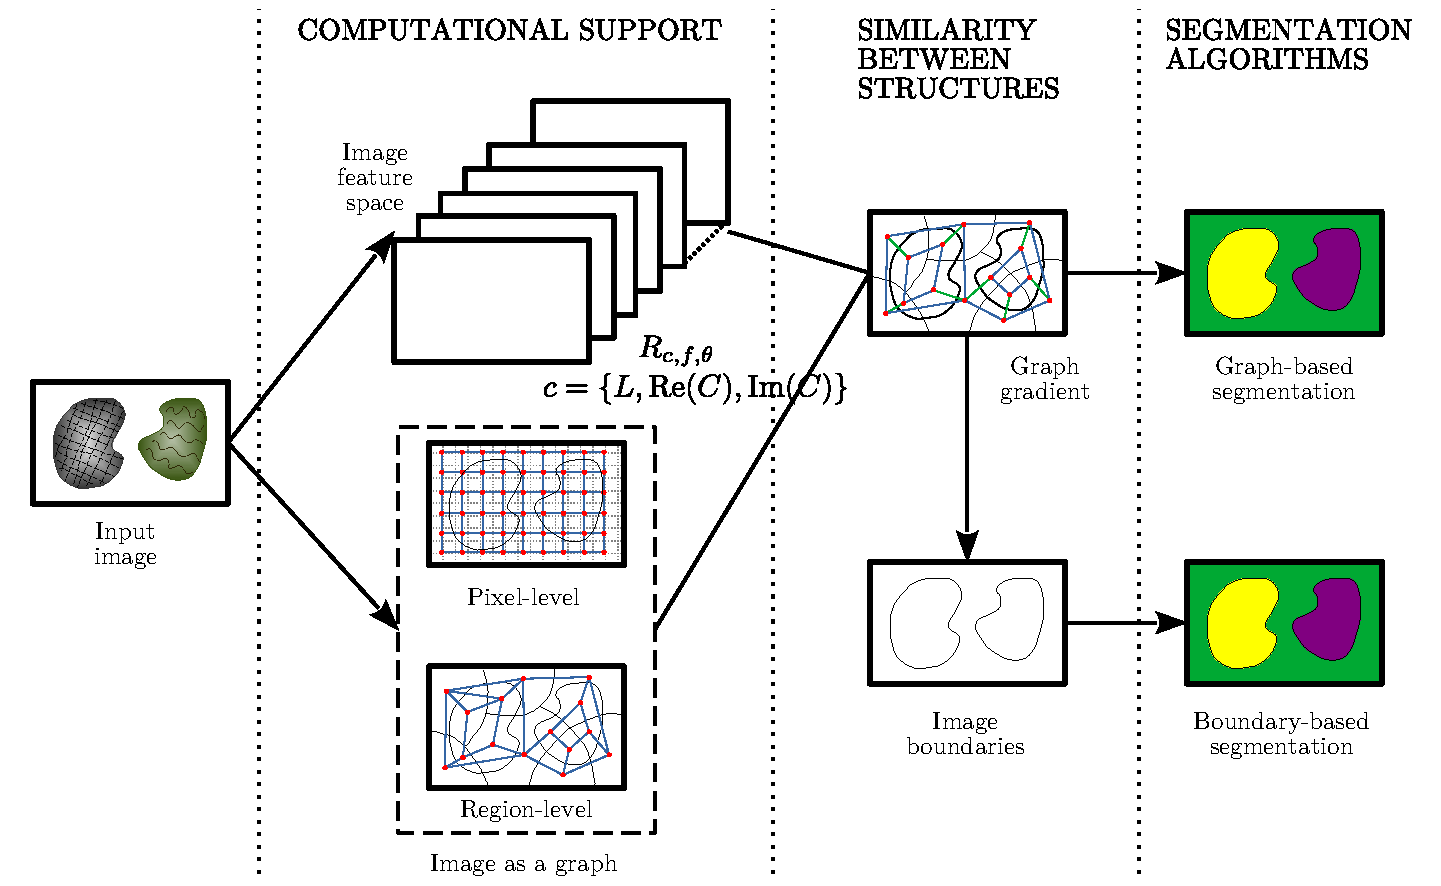
\includegraphics[width=\textwidth]{img_boundaries_segmentation_diagram}
	\caption{General pipeline for extraction of perceptual image boundaries and unsupervised image segmentation.}\label{fig:pipeline_gabor_image_segmentation}
\end{figure}

\section{Related Work}\label{sec:soa_boundaries_segmentation}
Edge detection is a fundamental problem of computer vision that has been intensively studied since the early 1970s \citep{Hueckel:JACM:1971, Fram.Deutsch:TC:1975}. The main idea behind traditional approaches to contour extraction is to model edges as discontinuities in the brightness channel of an image. This idea gave way to the creation of mask-based operators such as Sobel \citep{Sobel.Feldman:SAIL:1990}, Roberts \citep{Roberts:Thesis:1963}, Gradient \citep{Maitre:Book:2003} and Prewitt \citep{Prewitt:PPP:1970}, which quantify the presence of an edge through the convolution of a gray level image with local derivative filters. Other techniques, such as Marr and Hildreth \citep{Marr.Hildreth:PRS:1980}, define edges as the zero crossings of the Laplacian of a Gaussian (LoG). The Canny operator \citep{Canny:PAMI:1986} is one of the most popular approaches to this day within traditional methods. This operator follows the same operation principle of the previous methods, adding a non-maximum suppression stage and hysteresis thresholding. 

Despite their efficiency in controlled environments or synthetic images, traditional methods suffer from identifying contours in natural images. The edges of natural images can be present at different scales, and the colors and textures of the scene can generate edges that are perceptually significant to the human eye. Ideally, a contour detection method is intended to simultaneously exploit the brightness, color, and texture properties of an image so that it can handle the boundary perimeters defined by the brightness steps and the regions with consistent color and (or) texture.

One of the relatively recent strategies for identifying perceptual contours is to use the local energy response of an image. The operation principle is simple: generate features from the responses of an image produced by a family of filters at different scales and orientations. The idea has been exploited from different points of view. For example, the use of the Difference of Gaussians (DoG) and its Hilbert transform \citep{Morrone.Owens:PR:1987, Morrone.Burr.ea:RSL:1988} to generate a family of filters. Inspired by Gabor's work, this group of filters comply with the Parseval principle and generate an exact quadrature pair (even and odd symmetry cells). 

The \textit{Probability-of-boundary} (Pb) detector \citep{Malik.Belongie.ea:IJCV:2001} is one of the principal exponents of using a filter bank formed by the DoG and its Hilbert transform. The contour detector only uses the brightness and texture information to obtain the Pb. The brightness information is processed following the intervening contour framework \citep{Leung.Malik:ECCV:1998}, which consists of obtaining the image's quadrature energy, also called oriented energy (OE). The texture information is analyzed using so-called textons \citep{Malik.Belongie.ea:ICCV:1999}. Since each cue (brightness and texture) has a domain of applicability, hence different units of magnitude, they introduce a gating operator based on a neighborhood's texturedness at a pixel. The operator gives, as a result, a local measure that indicates how much two nearby pixels are to belong to the same region. Later in that work, they use spectral graph theory (normalized cut algorithm \citep{JianboShi.Malik:PAMI:2000}) to segment the image into coherent texture and brightness regions. 

This contemporary method, developed by the UC Berkeley research group, was the basis for many other techniques for contour detection and segmentation of natural images widely used today. Most of these works bring substantial improvements to the Pb detector. For example, the seminal papers \citep{Martin.Fowlkes.ea:NIPS:2002} and \citep{Martin.Fowlkes.ea:PAMI:2004} bring together previous works related to Pb and obtain a feature space of four image characteristics: localized OE, Brightness Gradient (BG), Color Gradient (CG), and localized Texture Gradient (TG). To cope with the difference in units of the magnitude of the cues, they use a logistic regression classifier to combine oriented energy, brightness, color, and texture. The proposed supervised method optimizes each feature's weights, formulating it as a two-class classification problem, where they learn the rules for combining cues from the ground truth data of the Berkeley Segmentation Dataset (BSDS) \citep{Martin.Fowlkes.ea:ICCV:2001}.

On the other hand, \cite{Ren:ECCV:2008} showed that the Pb detector improves when using features of the image calculated at different scales. However, a better version of the Pb detector, which has dominated the state of the art scores for several years, is obtained by combining local and global contours \citep{Maire.Arbelaez.ea:CVPR:2008}. The local contours are represented by the multiscale oriented signal mPb, while the global contours are represented by the oriented signal from the spectral partition sPb. The final detector that combines both signals is the globalized Probability-of-boundary gPb, which learns the local and global part's weights through an ascending gradient, taking as reference the BSDS evaluation score.

The Berkeley research group laid the foundation for contour detection and natural image segmentation, providing quantitative comparison methods. However, there are other methods in the literature that use different strategies to calculate image features and detect contours. Such methods can usefully supervise approaches, avoiding the careful hand-drawing of texture and gloss gradients. However, we can also find semi-supervised methods that replace the Pb detector to apply later a preprocessing chain similar to that applied in the Berkeley group methods.

The Berkeley research group laid the foundation for contour detection and natural image segmentation, providing the database and tools for the comparison and quantitative evaluation of the different approaches. Furthermore, Pb has motivated the development of state-of-the-art methods that use different strategies to obtain image features and contour detection. Such methods can use supervised approaches, avoiding careful filter design, computation of texture and brightness gradients, and hand-crafted features. We can also find semi-supervised methods, which generally replace the Pb detector with a supervised detector to apply later a preprocessing chain similar to that applied in the Berkeley group methods to refine the detection.

The set of the most popular supervised methods for contour detection, led by researchers from the University of Pasadena California and colleagues, is based on the calculation of features on channels of integrals of the image \citep{Dollar.Tu.ea:BMVC:2009}. Some examples of these integral channels are image color and gray channels, image responses to linear filters (e.g., Gabor filters, DoG), non-linear image transformations (e.g., Canny edges, gradient magnitude, hysteresis threshold), among others. The calculation of features on the integral channels follows the object detection framework of \cite{Viola.Jones:IJCV:2004}, obtaining first-order and higher-order features such as Haar-like features. Following this principle, a pool of features is obtained by randomly choosing both the integral channel and a rectangle where the features are calculated, allowing the acceleration of the computation of features and boosting learning techniques. 

Some of the supervised edge detectors that use the integral channel features as input are the Boosted Energy Learning (BEL) \citep{Dollar.ZhuowenTu.ea:CVPR:2006}, which attempts to learn an edge classifier in the form of a probabilistic boosting tree from the thousands of simple features calculated in image patches. On the other hand, Sketch tokens \citep{Lim.Zitnick.ea:CVPR:2013} uses the same features as input to a random forest classifier. The peculiarity of this second method is that the classes of the classifier are the so-called sketch tokens; mid-level information patches that represent complex shapes such as joints, corners, vertical and horizontal edges, calculated from the contours of the ground truth. The Structural Edge (SE) detector \citep{Dollar.Zitnick:ICCV:2013} and its different versions \citep{Dollar.Zitnick:PAMI:2015} take these strategies to another level, learning not only the integral input features but also the output space, using structured-output decision forests. The Oriented Edge Forest (OEF) detector \citep{Hallman.Fowlkes:CVPR:2015} outperforms existing supervised methods using a decision forest that analyzes local patches and outputs probability distributions over the space of oriented edges passing through the patch. Finally, the detector based on a Deep Neural Network (DeepNet) architecture \citep{Kivinen.Williams.ea:PMLR:2014}, is a fully supervised method that does not use the framework of the integral features; instead, it calculates complex-cell like covariance features from multiple scales and semantic levels, which depend on the squared response of a filter to the input image. 

Another group of approaches to contour detection are those based on sparse local coding. Such techniques are said semi-supervised because they contain two main stages, one unsupervised and the other supervised. The first stage consists of obtaining a generic representation (without information of the contours) from the image's information in an unsupervised way. The second stage consists of transforming the sparse representation of the image into a classification task, wherein the case of contours detection is a two-classes supervised problem to label the pixels as a contour or no contour. Some renowned works under this approach are the detector proposed by \cite{Mairal.Leordeanu.ea:ECCV:2008} and the Sparse Code Gradients (SCG) detector \citep{Ren.Bo:NIPS:2012}. Both works use K-SVD as a dictionary learning algorithm and Orthogonal Matching Pursuit for efficient optimization and sparse coding of each pixel. At the end of the process, they use SVM as a linear classifier on the feature vectors resulting from the reconstruction error with each dictionary for pixel classification. The main difference between these detectors is that the SCG adopts the same scheme as the Pb detector, replacing the brightness, color, and texture gradients with sparse code gradients. Finally, the Sparse Code Transfer (SCT) detector \citep{Maire.Yu.ea:ACCV:2014} improves on the detector of \cite{Mairal.Leordeanu.ea:ECCV:2008} using a larger number of dictionaries at different scales and layers in addition to the multipath sparse coding technique, which rectifies the initial sparse codes to reconstruct the contours with an extra transfer dictionary. The main disadvantage of these semi-supervised methods is the computational time of both processes, dictionary calculation, and learning. 

There is a fine line between contour detection and image segmentation. In this sense, the Pb contour detector has also influenced image segmentation. The Ultrametric Contour Maps (UCM) \citep{Arbelaez.Maire.ea:PR:2009} uses the gPb to define a measure of dissimilarity (ultrametric distance) between pairs of adjacent regions defined by a hierarchical segmentation operator (HSO). This technique is refined by adding a supplementary preprocessing stage using the oriented watershed transform (OWT), giving rise to the gPb-owt-ucm hierarchical segmentation method \citep{Arbelaez.Maire.ea:PR:2009}. The extensive qualitative and quantitative comparison of these techniques can be consulted in \citep{Arbelaez.Maire.ea:PAMI:2011}.

The Pb contour detector has driven (directly or indirectly) 50 years of research work around perceptual contours detection in natural images and their segmentation. Like the Canny operator, the Pb operator has become a reference work. The importance of this method is that it provides a reasonable basis that considers human perception principles, using operators that have a physical sense. 


\section{Image as a Graph}

Graphs are mathematical structures that have been applied to almost all fields of engineering. Historically, Euler used these structures to solve a problem related to the optimal crossing of people across bridges. The success of these structures in fields such as electricity and chemistry contributed to creating a standard nomenclature, giving way to the Graph theory. 

Fundamentally, a graph is a helpful structure for modeling pairwise relations between objects. In this section, we present the notation and the commonly encountered graphs in image processing applications. 


%In the field of image processing we can find several approaches that make use of graphs. Generally these methods solve a minimization problem. For example, the \textit{minimun spanning tree} approach that aims to find for each pair of nodes, the path with the least weight edges. On the other hand, the \textit{max-flow min-cut} approach aims to maximize flow with the minimum number of cuts in the graph. Both strategies have been successfully applied to the image segmentation problem. Another application example involves the algebraic theory of graphs that studies the spectrum of matrices that represent graphs.



\subsection{Graph Notations and Definitions}

This section introduces some critical definitions that will be used throughout the chapter related to graphs and related structures. 

\theoremstyle{definition}
\begin{definition}[Graph]
	A graph $\mathcal{G}$ is defined by the (assumed finite) sets $(\mathsf{V}, \mathsf{E})$ in which $\mathsf{E} \subset \mathsf{V} \times \mathsf{V}$. The elements of $\mathsf{v} \in \mathsf{V}$ are called \textit{vertices} and the elements of $\mathsf{e} \in \mathsf{E}$ are called edges. Since the edges are subsets of two nodes, we can write them as $\mathsf{e}_{i,j}$, $\{i, j\}$ or $\{\mathsf{v}_{i}, \mathsf{v}_{j}\} \quad \forall i, j \in \mathsf{V}$.
\end{definition}

\begin{definition}[Subgraph]
	A subgraph $\mathcal{G}'= (\mathsf{V}', \mathsf{E}')$ is a (partial) graph of $\mathcal{G}=(\mathsf{V}, \mathsf{E})$ if $\mathsf{V}' \subseteq \mathsf{V}$, and  $\mathsf{E}'= \{\mathsf{e}_{i,j} \in \mathsf{E}\ |\ \mathsf{v}_i,\mathsf{v}_j \in \mathsf{V}' \}$.
\end{definition}

\begin{definition}[Edge-weighted graph]
	Given a graph $\mathcal{G}=(\mathsf{V}, \mathsf{E})$, egde weighting is a function $\omega: \mathsf{E} \rightarrow \mathbb{R}$. The weight of an edge incident to two vertices is denoted by  $\omega(\mathsf{v}_{i}, \mathsf{v}_{j})$, $ \omega(\mathsf{e}_{i,j})$ or simply as $\omega_{i,j}$. We denote an edge-weighted graph as $(\mathcal{G}, \omega)$.
\end{definition}

\begin{definition}[Node-weighted graph]
	Given a graph $\mathcal{G}=(\mathsf{V}, \mathsf{E})$, vertex weighting is a function $\hat{\omega}: \mathsf{V} \rightarrow \mathbb{R}$. The weight of a vertex is denoted by  $\hat{\omega}(\mathsf{v}_{i})$ or simply as $\hat{\omega}_{i}$. We denote a node-weighted graph as $(\mathcal{G}, \hat{\omega})$.
\end{definition}

\begin{definition}[Adjacency]
	Given an edge $\mathsf{e}_{i,j}$ that connects $\{\mathsf{v}_{i}, \mathsf{v}_{j}\} $, the two vertices $\{\mathsf{v}_{i}, \mathsf{v}_{j}\}$ contained in the edge are said to be \textit{adjacent} or \textit{neighbors}. In the same way two edges that share a vertex are \textit{adjacent}.
\end{definition}

\begin{definition}[Neighborhood]
	Given a graph $\mathcal{G}=(\mathsf{V}, \mathsf{E})$, a neighbourhood $N_i$ is the subgraph of $\mathcal{G}$ containing all adjacent vertices of $\mathsf{v}_i$.
\end{definition}

\begin{definition}[Adjacency matrix]
	The adjacency matrix of a graph $\mathcal{G}=(\mathsf{V}, \mathsf{E})$ is a $|\mathsf{V}| \times |\mathsf{V}|$ matrix $A_{\mathcal{G}}$ that indicates whether pairs of vertices are adjacent or not. For undirected graphs, it is a symmetric $(0,1)$-matrix with zeros on its diagonal such that 
	
	\begin{equation}	
		A_{\mathcal{G}} = (A_{ij})_{(i, j)\in \{1,\cdots, n\}}  \quad \text{where $n=|\mathsf{V}|$ is the number of nodes in $\mathcal{G}$ and} \nonumber 		
	\end{equation}
	\begin{equation}	
		A_{ij}= 
		\begin{cases}
			1 \quad \text{if $i, j$ are adjacent in $\mathcal{G}$} \\
			0 \quad \text{elsewhere}
		\end{cases}		\nonumber		
	\end{equation}
	The adjacency matrix may be transformed into a weighted adjacency matrix $W$ replacing the 1 by the edge weight $\omega_{ij}$ if $i, j$ are adjacent.
\end{definition}

\begin{definition}[Affinity matrix]
	The affinity matrix $A$ (also called similarity matrix) of a graph $\mathcal{G}=(\mathsf{V}, \mathsf{E})$ is a $|\mathsf{V}| \times |\mathsf{V}|$ matrix that indicates how affine or similar a pair of vertices are. For undirected graphs, it is a symmetric matrix with zeros on its diagonal such that 
	
	\begin{equation}	
		A = (A_{ij})_{(i, j)\in \{1,\cdots, n\}}  \quad \text{with}  \nonumber 		
	\end{equation}
	\begin{equation}	
		A_{ij}= 
		\begin{cases}
			s(i,j) \quad \text{if $i, j$ are adjacent in $\mathcal{G}$} \\
			0 \quad \text{elsewhere}
		\end{cases}	 \nonumber		
	\end{equation}
where $n=|\mathsf{V}|$ is the number of nodes in $\mathcal{G}$ and $s(i,j)$ is some strictly positive similarity function between the points $i,j$.
\end{definition}

\begin{definition}[Degree matrix]
	The Degree matrix $D=(D_{ij})$ is a diagonal matrix that measures the \textit{degree} at each node $\mathsf{v} \in \mathsf{V}$ of a graph $\mathcal{G}$ such that 
	\begin{equation}	
		D_{ii} =  \underset{\{j|(i,j)\in \mathsf{E}\}}{\sum}  s(i,j)  \nonumber 		
	\end{equation}	
\end{definition}

\begin{definition}[Laplacian matrix]
	Given a graph $\mathcal{G}$ with $n=|\mathsf{V}|$ vertices, its Laplacian matrix $L = (L_{ij})_{(i, j)\in \{1,\cdots, n\}}$ is defined as 
	\begin{equation}	
		L = D - A  \nonumber 		
	\end{equation}	
where $D$ is the degree matrix and $A$ is the affinity matrix of the graph.
\end{definition}

\begin{definition}[Minimum Spanning Tree (MST)]
	Given an edge-weighted graph $\mathcal{G}=(\mathsf{V}, \mathsf{E})$, the minimum spanning tree is a subset of edges that connects all the nodes together with the minimum possible total edge weight. That is, is a spanning tree $\mathcal{MST}=(\mathsf{V}, \mathsf{E}_{MST})$ of $(\mathcal{G}, \omega)$ such that
the sum of its edges is minimal.

\begin{equation}
	\mathcal{MST}(\mathcal{G}) = \underset{\mathcal{T} \in \mathcal{ST}}{\mathrm{argmin}} \left( \sum_{\mathsf{e}_{i,j} \in \mathsf{E}_\mathcal{ST}} \omega_{ij} \right) \nonumber
\end{equation}
where $\mathcal{ST}$ is the set of all trees $\mathcal{T}$ of $\mathcal{G}$.
\end{definition}

\begin{definition}[Graph cut]
	A cut $\mathsf{C}=(\mathsf{S}, \mathsf{T})$ is a partition of the vertices $\mathsf{V}$ of a graph $\mathcal{G}=(\mathsf{V}, \mathsf{E})$ into two disjoint subsets $\mathsf{S}$, $\mathsf{T}$. The set nodes of a graph cut is denoted as $\mathsf{C}=\{ (\mathsf{s}, \mathsf{t}) \in \mathsf{E} | \mathsf{s} \in \mathsf{S}, \mathsf{t} \in \mathsf{T} \}$.
\end{definition}
%

\subsubsection{Pixel-based graph representation}

Considering a digital image as a 2-d grid of pixels, where the intensity (or color) values are mapped to the spatial coordinates $(x, y)$, we can use the graph theory to represent all the pixels as a dense graph. In the graph notation $\mathcal{G}=(\mathsf{V}, \mathsf{E})$, each node $\mathsf{v}_i \in \mathsf{V}$ corresponds to a pixel in the image, and the edges $\mathsf{e} \in \mathsf{E}$ the link between the image's pixels.

There are several strategies to link the nodes of a graph. The types of graphs that we can form are a function of such linking strategies. For example, the complete graph connects each pair of different nodes with a single edge. The epsilon-graph connects a pair of nodes if they are within an epsilon distance. The k-nearest neighbors' graph (knn-graph) connects a central node to another node only if the distance between them is among the k smallest distances from the central node to other nodes. Lastly, the adjacency graph connects only a pair of nodes if they are neighbors or adjacent. At a pixel level, this last graph is referred to as a  \textit{Pixel Adjacency Graph} (PAG).

We can define the adjacency level of the pixels to generate a specific pixel-based graph. In our applications, we mainly use the 4-neighbor adjacency system. This configuration and other adjacency systems based are illustrated in figure \ref{fig:pixel_adjacency_graph}.


\begin{figure}[!ht]
    \centering

	\begin{subfigure}[b]{0.2\textwidth}
    	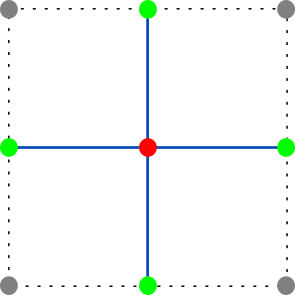
\includegraphics[width=\textwidth]{4nn_pag}
        \caption{ 4-neighborhood}
    \end{subfigure}\qquad   
    \begin{subfigure}[b]{0.2\textwidth}
    	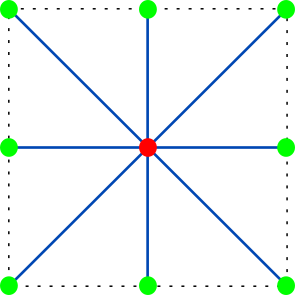
\includegraphics[width=\textwidth]{8nn_pag}
        \caption{8-neighborhood}
    \end{subfigure}\qquad
    \begin{subfigure}[b]{0.23\textwidth}
    	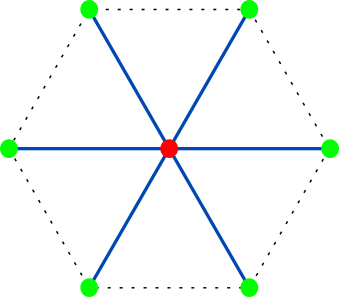
\includegraphics[width=\textwidth]{6nn_pag}
        \caption{6-neighborhood}
    \end{subfigure}\\[5ex]    
    \begin{subfigure}[b]{0.5\textwidth}
        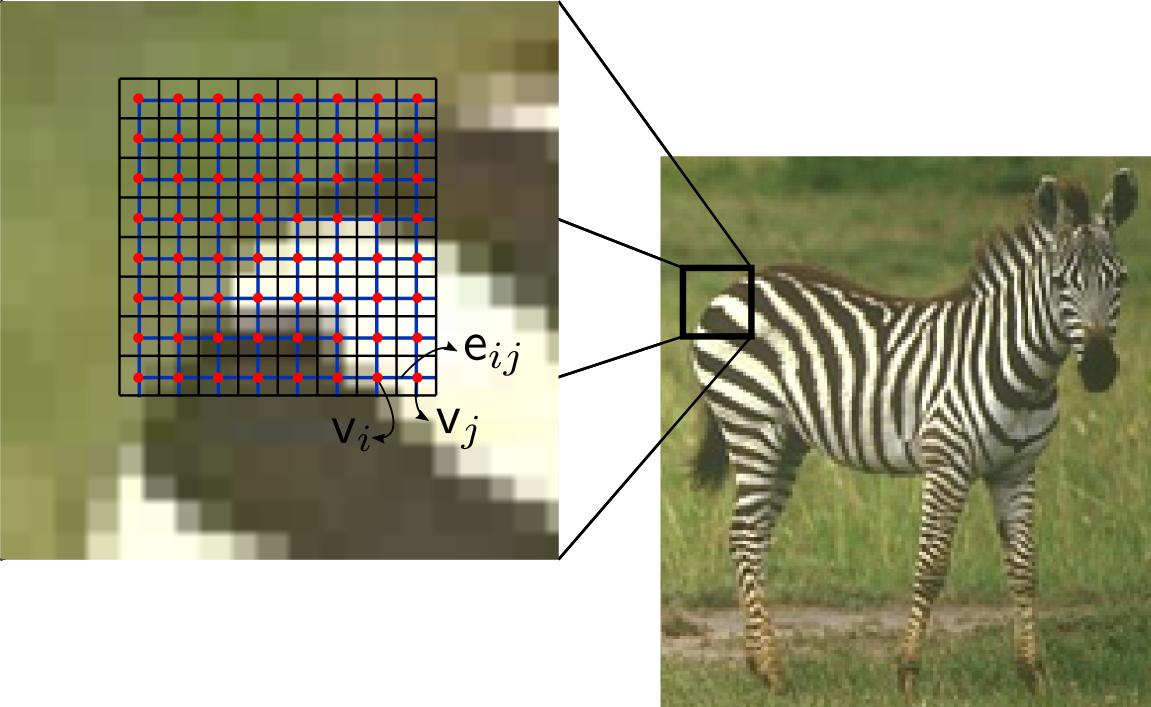
\includegraphics[width=\textwidth]{pixel_adjacency_graph}
        \caption{Exaple of a 4-n graph on a real image}
        \label{fig:pag_example}
    \end{subfigure}         
        	    
    \caption{Most common k-nearest neighbors adjacency systems.}\label{fig:pixel_adjacency_graph}    
\end{figure}

The representation of an image as a graph opens the possibility of new methods for data processing; however, a recurring problem is the need to satisfy the compromise between algorithmic complexity and precision. In most algorithms, complexity is a function of the number of nodes and edges in the graph, so the adjacency system plays an essential role in the speed of the methods applied to an image graph. One way to reduce the number of nodes (and consequently the number of edges) is to use graphs on the image's elements of greater size.

\subsubsection{Region-based graph representation}

To build this type of graph, we must first separate the image into regions, preferably into regions that are coherent with the image's perceptual information. Subsequently, the graph nodes represent the image regions while the graph edges follow the same strategies described above to connect the regions. The primary type of graph that we consider in this work is the \textit{Region Adjacency Graph }(RAG).


\begin{figure}[!ht]
	\centering
	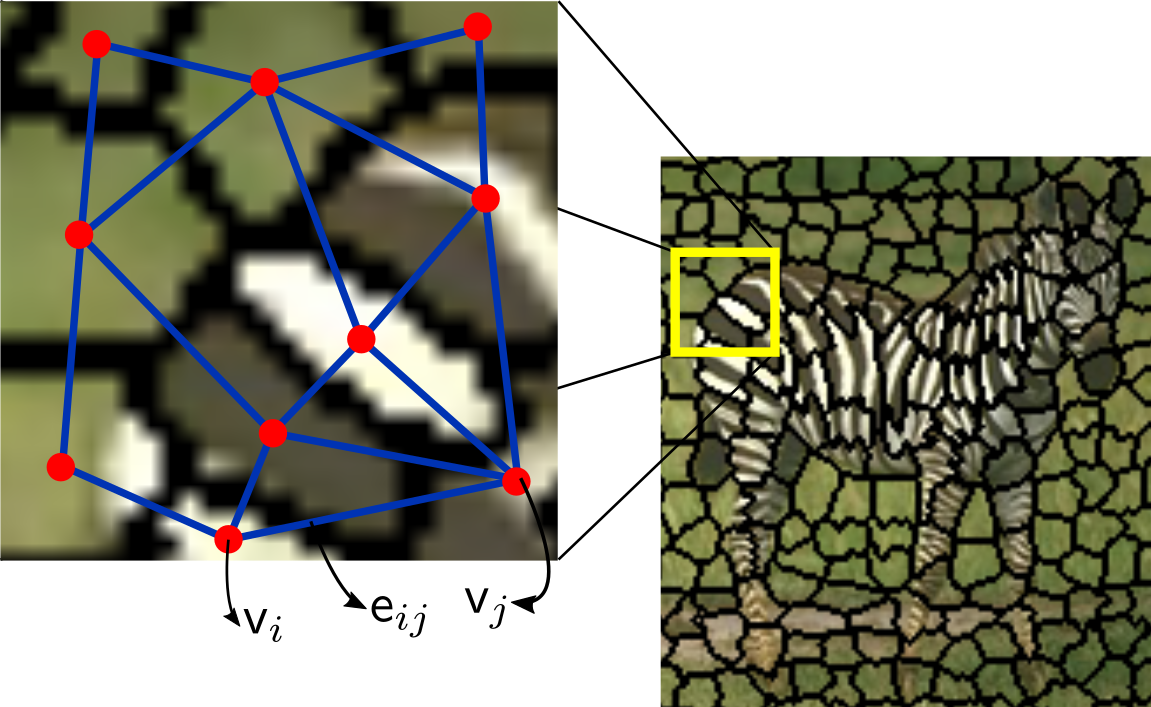
\includegraphics[width=0.5\textwidth]{region_adjacency_graph}       	    
    \caption{Example of a Region Adjacency Graph on a real image.}
    \label{fig:region_adjacency_graph}    
\end{figure}


Pixels are the smallest elements in the image. The grouping of these elements into coherent regions generates the so-called superpixels. In the following section, we introduce some of the most used methods for generating these regions, exposing their main characteristics.


\subsection{Superpixels}

Pixels are a consequence of the discrete representation of the intensity or color of an image; therefore, pixels are not entities that naturally reflect the perceptual information in an image. Moreover, the number of pixels on an image is too high (even in moderate resolutions), making the optimization at pixel level difficult. The superpixels are locally coherent and preserve most of the structure necessary for image processing algorithms.

The term \textit{superpixels} was introduced first by \cite{Ren.Malik:ICCV:2003} o describe the resulting regions of an over-segmentation image process. However,  \cite{Stutz.Hermans.ea:CVIU:2018} gathers a series of requirements from different state-of-the-art works to differentiate superpixels from other regions generated by over-segmentation algorithms. 

\begin{itemize}
 \item \textbf{Partition}. Superpixels should define a partition of the image. They should be disjoint and assign a label to every pixel.
 \item \textbf{Connectivity}. Superpixels represent a connected set of pixels.
 \item Boundary Adherence. Superpixels must preserve image boundaries.
 \item \textbf{Compactness, Regularity and Smoothness}. Superpixels should be compact (closed and bounded), placed regularly, and exhibit smooth boundaries.
 \item \textbf{Efficiency}. Superpixels should be generated efficiently

 \item \textbf{Controllable number of superpixels}. The number of superpixels should be controllable.
\end{itemize}

Besides, according to the followed strategy to obtain the regions, \cite{Stutz.Hermans.ea:CVIU:2018} propose a classification for superpixels techniques. We present four superpixel techniques; each one of them represents a category of the classification.


%\begin{enumerate}
% \item \textbf{Watershed-based.} Based on the watershed algorithm, these methods generally depends on a image pre-processing step and the markers setting. 
% \item \textbf{Density-based.} Perform mode-seeking in a computed density image. These methods usually do not offer control over the number of superpixels or their compactness (they are consider as oversegmentation algorithms). 
% \item \textbf{Graph-based.} Treat the image as undirected graph and do a the image partition based on edge-weights  (computed as color differences or similarities).
% \item \textbf{Clustering-based.} Inspired in clissical clustering methods (k-means), these techniques group the pixels from seed pixels using color information, spacial information, and other (such as depth information). The number of superpixels and their compactness is controllable.
%\end{enumerate}


\subsubsection{Felzenszwalb's Superpixels}

This technique belongs to the category of graph-based superpixels, representing the region generation problem in terms of an edge-weighted undirected graph.

This method treats the image as an undirected graph and produces the image partition based on edge-weights (computed as color differences or similarities) \citep{Felzenszwalb.Huttenlocher:IJCV:2004}. We can obtain the weight of an edge $\omega_{ij}$
in two ways:
\begin{enumerate}
	\item $\omega(\mathsf{v}_i, \mathsf{v}_j)= I(p_i) - I(p_j)|$, the absolute intensity difference between the pixels connected by an edge; 
	\item $\omega(\mathsf{v}_i, \mathsf{v}_j)= X(p_i) - X(p_j)|$, the L2 (Euclidean) distance between two corresponding pixels in the feature space.
\end{enumerate}

For color images, it is possible to use option 1, considering each color channel as an individual intensity channel, and then combine the tree weights. Otherwise, the feature space of option 2 is defined by $X = (x, y,r, g, b)$, where $(x, y)$ is the location of the pixels in the image and $(r, g, b)$ is the color value of the pixels. This method uses a Gaussian filter to smooth the image before the edge weights computation to compensate for digitization artifacts. 

Whit this method, we cannot directly control the number of resulting superpixels. We must use the Gaussian scale parameter to modify the size and shape of the superpixels. However, the actual size and number of segments can vary greatly, depending on local contrast.

\begin{figure}[!ht]
    \centering
    \begin{subfigure}[t]{\dimexpr0.2\textwidth+20pt\relax}
    	\makebox[20pt]{\raisebox{25pt}{ \rotatebox[origin=c]{90} {\small \textsf{\textbf{Input image}}} }}%
    	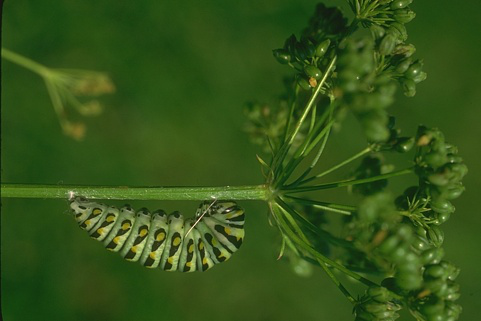
\includegraphics[width=\dimexpr\linewidth-20pt\relax]{35028} 
    \end{subfigure}      
    ~ %add desired spacing between images, e. g. ~, \quad, \qquad, \hfill etc. 
      %(or a blank line to force the subfigure onto a new line)
    \begin{subfigure}[b]{0.2\textwidth}
        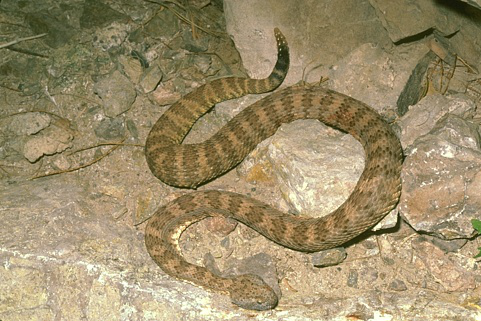
\includegraphics[width=\textwidth]{87015}
    \end{subfigure}
    ~ %add desired spacing between images, e. g. ~, \quad, \qquad, \hfill etc. 
      %(or a blank line to force the subfigure onto a new line)
    \begin{subfigure}[b]{0.2\textwidth}
        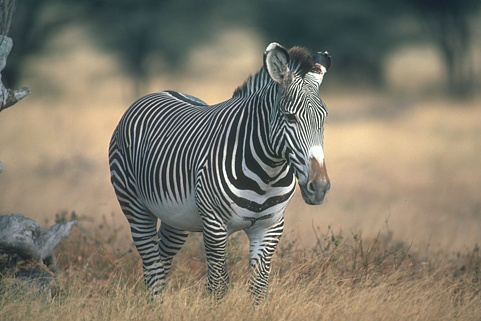
\includegraphics[width=\textwidth]{130066}
    \end{subfigure}
    ~ %add desired spacing between images, e. g. ~, \quad, \qquad, \hfill etc. 
      %(or a blank line to force the subfigure onto a new line)
    \begin{subfigure}[b]{0.2\textwidth}
        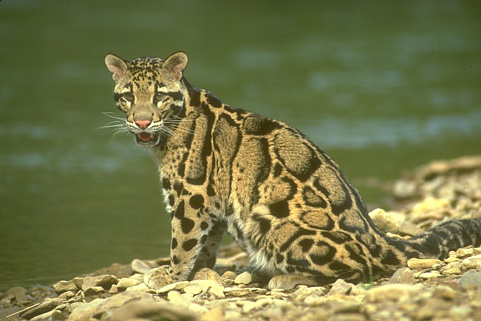
\includegraphics[width=\textwidth]{160067}
    \end{subfigure} \\[2ex]       
    
    \begin{subfigure}[t]{\dimexpr0.2\textwidth+20pt\relax}
    	\makebox[20pt]{\raisebox{25pt}{ \rotatebox[origin=c]{90} {\small \textsf{\textbf{150 sp}}} }}%
    	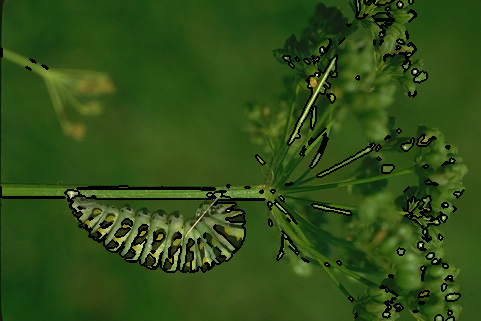
\includegraphics[width=\dimexpr\linewidth-20pt\relax]{35028_fz_150_segs} 
    \end{subfigure}      
    ~ %add desired spacing between images, e. g. ~, \quad, \qquad, \hfill etc. 
      %(or a blank line to force the subfigure onto a new line)
    \begin{subfigure}[b]{0.2\textwidth}
        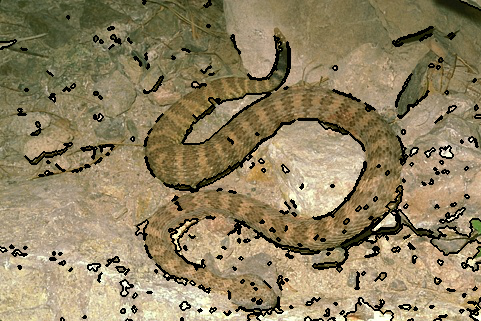
\includegraphics[width=\textwidth]{87015_fz_150_segs}
    \end{subfigure}
    ~ %add desired spacing between images, e. g. ~, \quad, \qquad, \hfill etc. 
      %(or a blank line to force the subfigure onto a new line)
    \begin{subfigure}[b]{0.2\textwidth}
        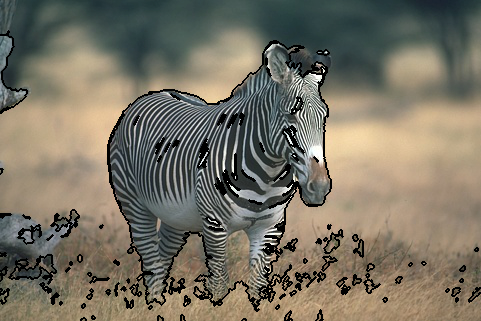
\includegraphics[width=\textwidth]{130066_fz_150_segs}
    \end{subfigure}
    ~ %add desired spacing between images, e. g. ~, \quad, \qquad, \hfill etc. 
      %(or a blank line to force the subfigure onto a new line)
    \begin{subfigure}[b]{0.2\textwidth}
        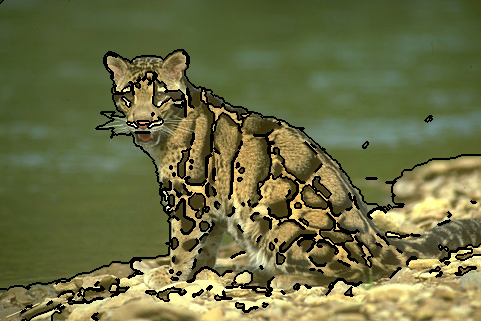
\includegraphics[width=\textwidth]{160067_fz_150_segs}
    \end{subfigure} \\ [2ex]
    
    \begin{subfigure}[t]{\dimexpr0.2\textwidth+20pt\relax}
    	\makebox[20pt]{\raisebox{25pt}{ \rotatebox[origin=c]{90} {\small \textsf{\textbf{300 sp}}} }}%
    	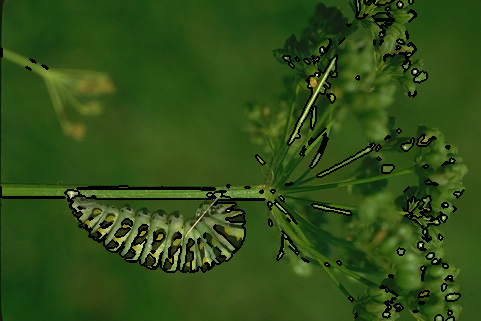
\includegraphics[width=\dimexpr\linewidth-20pt\relax]{35028_fz_150_segs} 
    \end{subfigure}      
    ~ %add desired spacing between images, e. g. ~, \quad, \qquad, \hfill etc. 
      %(or a blank line to force the subfigure onto a new line)
    \begin{subfigure}[b]{0.2\textwidth}
        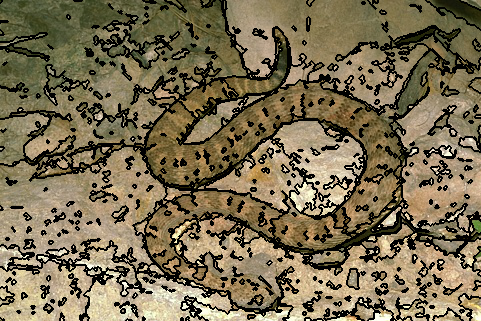
\includegraphics[width=\textwidth]{87015_fz_300_segs}
    \end{subfigure}
    ~ %add desired spacing between images, e. g. ~, \quad, \qquad, \hfill etc. 
      %(or a blank line to force the subfigure onto a new line)
    \begin{subfigure}[b]{0.2\textwidth}
        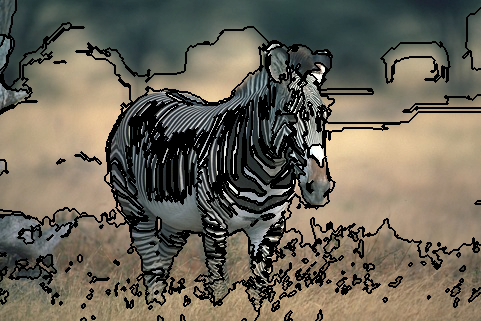
\includegraphics[width=\textwidth]{130066_fz_300_segs}
    \end{subfigure}
    ~ %add desired spacing between images, e. g. ~, \quad, \qquad, \hfill etc. 
      %(or a blank line to force the subfigure onto a new line)
    \begin{subfigure}[b]{0.2\textwidth}
        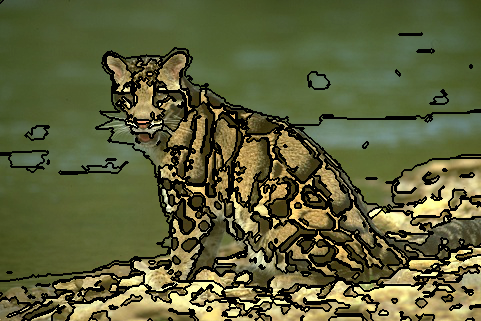
\includegraphics[width=\textwidth]{160067_fz_300_segs}
    \end{subfigure} \\ [2ex]
    
    \begin{subfigure}[t]{\dimexpr0.2\textwidth+20pt\relax}
    	\makebox[20pt]{\raisebox{25pt}{ \rotatebox[origin=c]{90} {\small \textsf{\textbf{600 sp}}} }}%
    	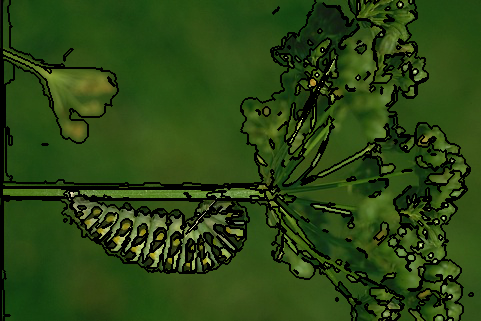
\includegraphics[width=\dimexpr\linewidth-20pt\relax]{35028_fz_600_segs} 
    \end{subfigure}      
    ~ %add desired spacing between images, e. g. ~, \quad, \qquad, \hfill etc. 
      %(or a blank line to force the subfigure onto a new line)
    \begin{subfigure}[b]{0.2\textwidth}
        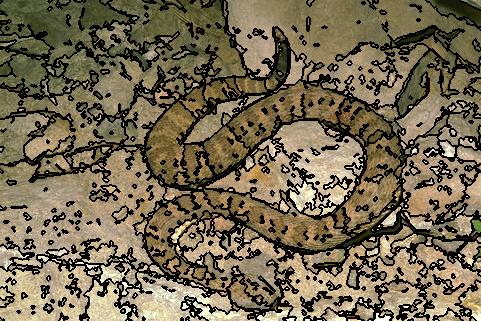
\includegraphics[width=\textwidth]{87015_fz_600_segs}
    \end{subfigure}
    ~ %add desired spacing between images, e. g. ~, \quad, \qquad, \hfill etc. 
      %(or a blank line to force the subfigure onto a new line)
    \begin{subfigure}[b]{0.2\textwidth}
        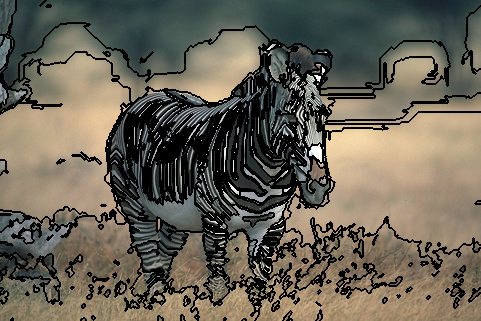
\includegraphics[width=\textwidth]{130066_fz_600_segs}
    \end{subfigure}
    ~ %add desired spacing between images, e. g. ~, \quad, \qquad, \hfill etc. 
      %(or a blank line to force the subfigure onto a new line)
    \begin{subfigure}[b]{0.2\textwidth}
        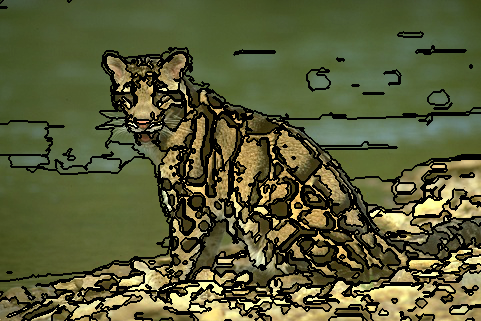
\includegraphics[width=\textwidth]{160067_fz_600_segs}
    \end{subfigure}     

	\caption{Examples of superpixels using Felzenszwalb's technique.}\label{fig:fz_suprepixels}    
\end{figure}

Figure \ref{fig:fz_suprepixels} shows the superpixels generated by adjusting the scale parameter to obtain approximately 150, 300, and 600 superpixels (sp). The examples show that Felzenszwalb's superpixel technique acts more like an over-segmentation algorithm since neither the size nor the regions' shape is close to being homogeneous.
 
\subsubsection{Quick shift superpixels} 

The Quick Shift (QS) \citep{Vedaldi.Soatto:ECCV:2008} is a density-based method for superpixel computation. This technique performs a so-called mode-seeking algorithm \citep{YizongCheng:PAMI:1995} for locating the maxima of a density function. It locates the maxima or the modes of a density function given discrete data sampled from that function through a mean shift procedure.

This superpixel technique is an iterative method that does not offer control over the number of superpixels or their compactness; therefore, it is also categorized as an over-segmentation algorithm.

The QS algorithm computes a hierarchical segmentation of the image at multiple scales simultaneously. The parameters to define the size and shape of the regions depend on the scale of the local density approximation and the level in the produced hierarchical segmentation. Additionally, we can also control the trade-off between color-space proximity and image-space proximity.

\begin{figure}[!ht]
    \centering
    \begin{subfigure}[t]{\dimexpr0.2\textwidth+20pt\relax}
    	\makebox[20pt]{\raisebox{25pt}{ \rotatebox[origin=c]{90} {\small \textsf{\textbf{Input image}}} }}%
    	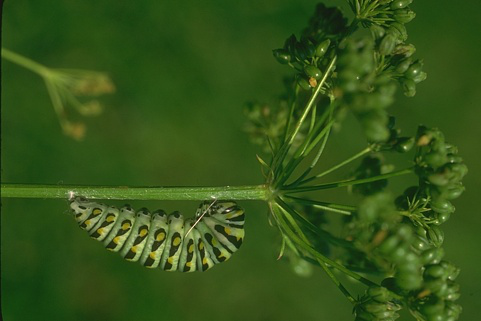
\includegraphics[width=\dimexpr\linewidth-20pt\relax]{35028} 
    \end{subfigure}      
    ~ %add desired spacing between images, e. g. ~, \quad, \qquad, \hfill etc. 
      %(or a blank line to force the subfigure onto a new line)
    \begin{subfigure}[b]{0.2\textwidth}
        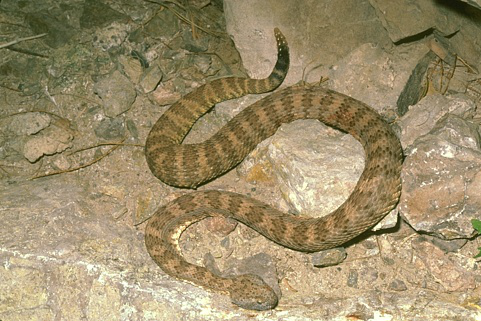
\includegraphics[width=\textwidth]{87015}
    \end{subfigure}
    ~ %add desired spacing between images, e. g. ~, \quad, \qquad, \hfill etc. 
      %(or a blank line to force the subfigure onto a new line)
    \begin{subfigure}[b]{0.2\textwidth}
        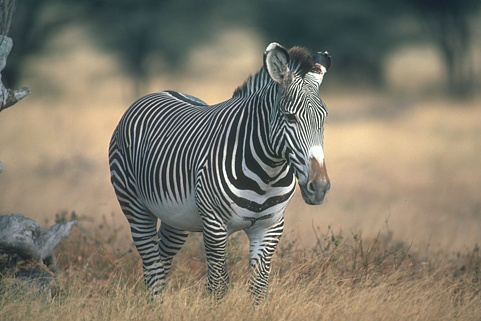
\includegraphics[width=\textwidth]{130066}
    \end{subfigure}
    ~ %add desired spacing between images, e. g. ~, \quad, \qquad, \hfill etc. 
      %(or a blank line to force the subfigure onto a new line)
    \begin{subfigure}[b]{0.2\textwidth}
        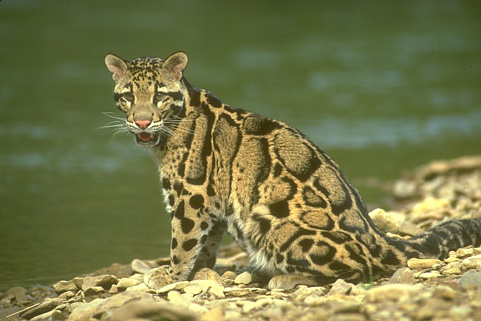
\includegraphics[width=\textwidth]{160067}
    \end{subfigure} \\[2ex]       
    
    \begin{subfigure}[t]{\dimexpr0.2\textwidth+20pt\relax}
    	\makebox[20pt]{\raisebox{25pt}{ \rotatebox[origin=c]{90} {\small \textsf{\textbf{150 sp}}} }}%
    	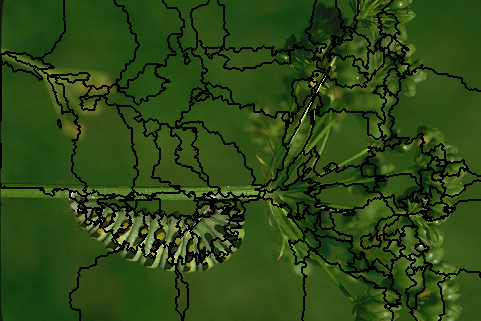
\includegraphics[width=\dimexpr\linewidth-20pt\relax]{35028_quick_150_segs} 
    \end{subfigure}      
    ~ %add desired spacing between images, e. g. ~, \quad, \qquad, \hfill etc. 
      %(or a blank line to force the subfigure onto a new line)
    \begin{subfigure}[b]{0.2\textwidth}
        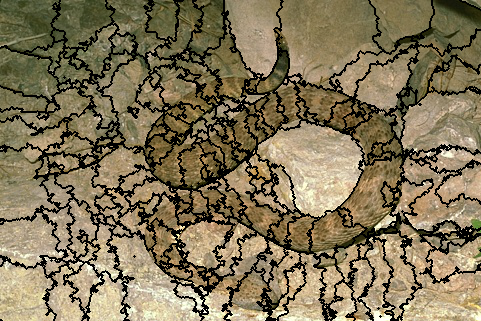
\includegraphics[width=\textwidth]{87015_quick_150_segs}
    \end{subfigure}
    ~ %add desired spacing between images, e. g. ~, \quad, \qquad, \hfill etc. 
      %(or a blank line to force the subfigure onto a new line)
    \begin{subfigure}[b]{0.2\textwidth}
        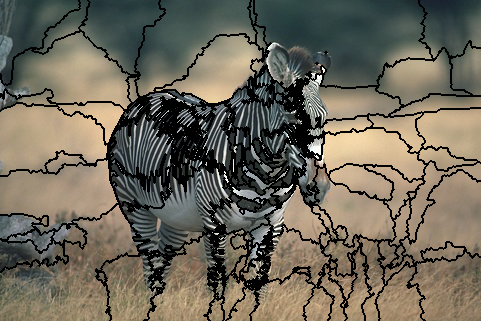
\includegraphics[width=\textwidth]{130066_quick_150_segs}
    \end{subfigure}
    ~ %add desired spacing between images, e. g. ~, \quad, \qquad, \hfill etc. 
      %(or a blank line to force the subfigure onto a new line)
    \begin{subfigure}[b]{0.2\textwidth}
        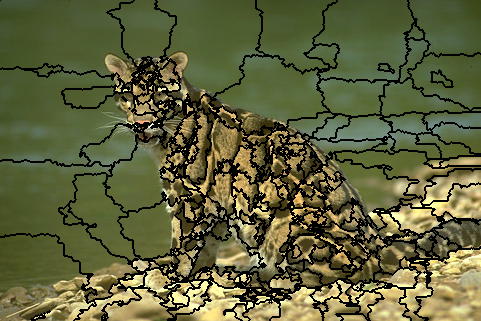
\includegraphics[width=\textwidth]{160067_quick_150_segs}
    \end{subfigure} \\ [2ex]
    
    \begin{subfigure}[t]{\dimexpr0.2\textwidth+20pt\relax}
    	\makebox[20pt]{\raisebox{25pt}{ \rotatebox[origin=c]{90} {\small \textsf{\textbf{300 sp}}} }}%
    	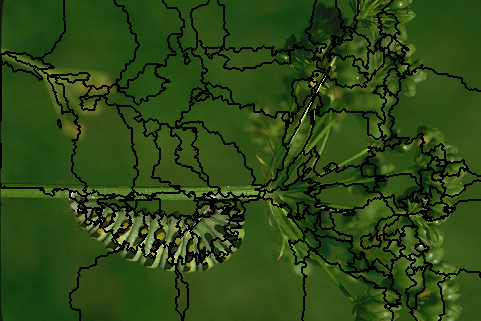
\includegraphics[width=\dimexpr\linewidth-20pt\relax]{35028_quick_150_segs} 
    \end{subfigure}      
    ~ %add desired spacing between images, e. g. ~, \quad, \qquad, \hfill etc. 
      %(or a blank line to force the subfigure onto a new line)
    \begin{subfigure}[b]{0.2\textwidth}
        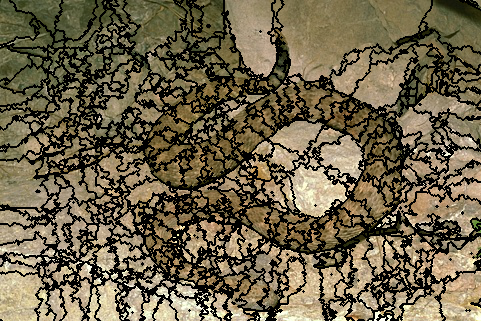
\includegraphics[width=\textwidth]{87015_quick_300_segs}
    \end{subfigure}
    ~ %add desired spacing between images, e. g. ~, \quad, \qquad, \hfill etc. 
      %(or a blank line to force the subfigure onto a new line)
    \begin{subfigure}[b]{0.2\textwidth}
        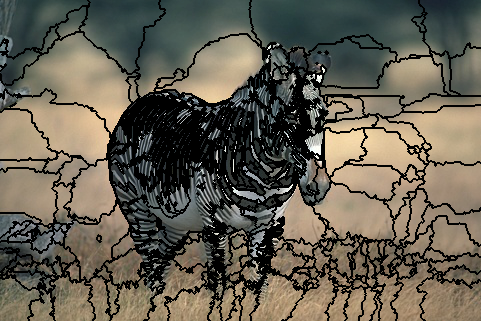
\includegraphics[width=\textwidth]{130066_quick_300_segs}
    \end{subfigure}
    ~ %add desired spacing between images, e. g. ~, \quad, \qquad, \hfill etc. 
      %(or a blank line to force the subfigure onto a new line)
    \begin{subfigure}[b]{0.2\textwidth}
        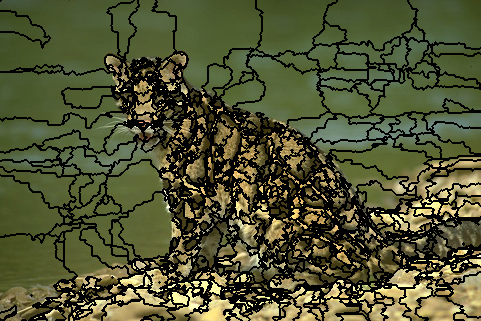
\includegraphics[width=\textwidth]{160067_quick_300_segs}
    \end{subfigure} \\ [2ex]
    
    \begin{subfigure}[t]{\dimexpr0.2\textwidth+20pt\relax}
    	\makebox[20pt]{\raisebox{25pt}{ \rotatebox[origin=c]{90} {\small \textsf{\textbf{600 sp}}} }}%
    	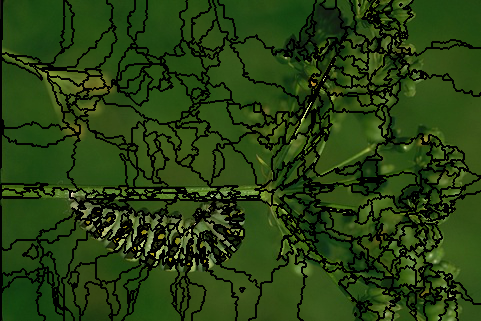
\includegraphics[width=\dimexpr\linewidth-20pt\relax]{35028_quick_600_segs} 
    \end{subfigure}      
    ~ %add desired spacing between images, e. g. ~, \quad, \qquad, \hfill etc. 
      %(or a blank line to force the subfigure onto a new line)
    \begin{subfigure}[b]{0.2\textwidth}
        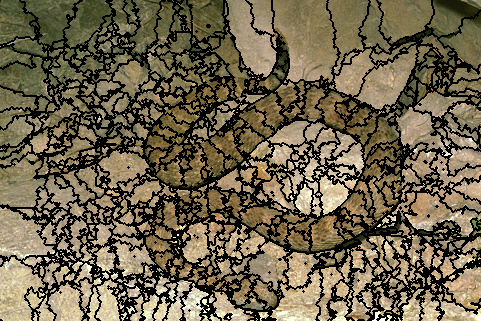
\includegraphics[width=\textwidth]{87015_quick_600_segs}
    \end{subfigure}
    ~ %add desired spacing between images, e. g. ~, \quad, \qquad, \hfill etc. 
      %(or a blank line to force the subfigure onto a new line)
    \begin{subfigure}[b]{0.2\textwidth}
        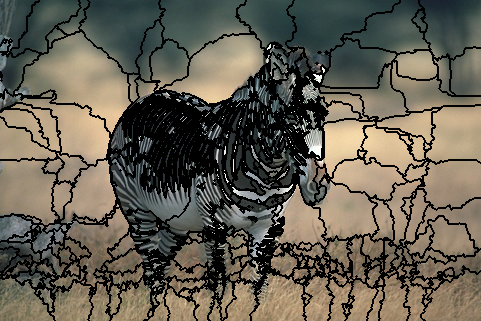
\includegraphics[width=\textwidth]{130066_quick_600_segs}
    \end{subfigure}
    ~ %add desired spacing between images, e. g. ~, \quad, \qquad, \hfill etc. 
      %(or a blank line to force the subfigure onto a new line)
    \begin{subfigure}[b]{0.2\textwidth}
        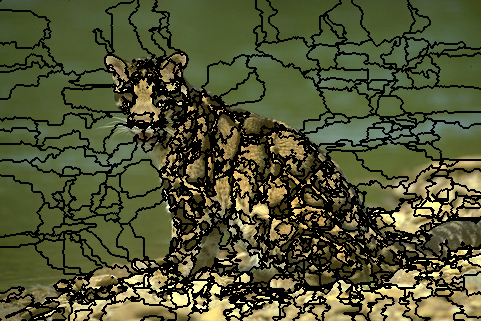
\includegraphics[width=\textwidth]{160067_quick_600_segs}
    \end{subfigure}     

	\caption{Examples of Quick Shift superpixels.}\label{fig:quick_suprepixels}    
\end{figure}

We illustrate in figure \ref{fig:quick_suprepixels} four images and the superpixels obtained with the QS algorithm setting the parameters to obtain 150, 300, and 600 superpixels. 


\subsubsection{Watershed superpixels}%Compact watershed segmentation of gradient images
The watershed-based superpixel techniques take the watershed segmentation algorithm proposed by \citep{Meyer:ICIP:1992} as a calculation basis. Initially, the watershed method is an over-segmentation technique, i.e., one can control the number of regions employing the number of markers, but we can not control its compactness. In this context, high compactness means that the superpixels are of approximately equal size and more or less regularly shaped in the absence of strong image gradients. Some watershed-based superpixel algorithms, such as the Compact watershed algorithm \citep{Neubert.Protzel:ICPR:2014} or the Water Pixels algorithm \citep{Machairas.Faessel.ea:IP:2015}, upgrades the original algorithm adding the compactness. 

Initially, these algorithms implement a seeded watershed segmentation (also called marker-controlled watershed). Markers can be determined manually or automatically using, for example, the local minima of the image gradient or the local maxima of the distance function to the background. Therefore, instead of taking a color image as input, watershed requires a grayscale gradient image, where bright pixels denote a boundary between regions.

Once the markers and the gradient are given, the algorithm views the image as a landscape, where bright pixels of the gradient forms high peaks. This landscape is then flooded from the given markers until separate flood basins meet at the peaks. Each distinct basin forms a different image segment.

Figure \ref{fig:wt_suprepixels} shows the superpixels obtained with the compact watershed algorithm \citep{Neubert.Protzel:ICPR:2014} defining the number of superpixels to find at 150, 300, and 600.


\begin{figure}[!ht]
    \centering
    \begin{subfigure}[t]{\dimexpr0.2\textwidth+20pt\relax}
    	\makebox[20pt]{\raisebox{25pt}{ \rotatebox[origin=c]{90} {\small \textsf{\textbf{Input image}}} }}%
    	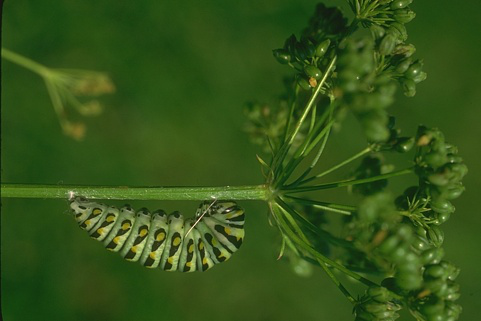
\includegraphics[width=\dimexpr\linewidth-20pt\relax]{35028} 
    \end{subfigure}      
    ~ %add desired spacing between images, e. g. ~, \quad, \qquad, \hfill etc. 
      %(or a blank line to force the subfigure onto a new line)
    \begin{subfigure}[b]{0.2\textwidth}
        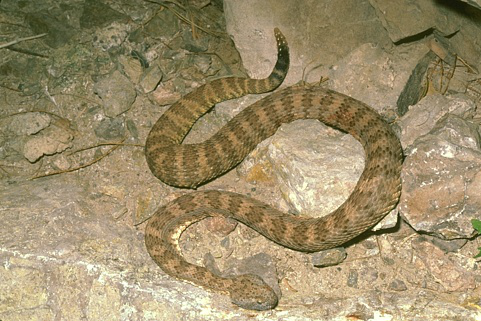
\includegraphics[width=\textwidth]{87015}
    \end{subfigure}
    ~ %add desired spacing between images, e. g. ~, \quad, \qquad, \hfill etc. 
      %(or a blank line to force the subfigure onto a new line)
    \begin{subfigure}[b]{0.2\textwidth}
        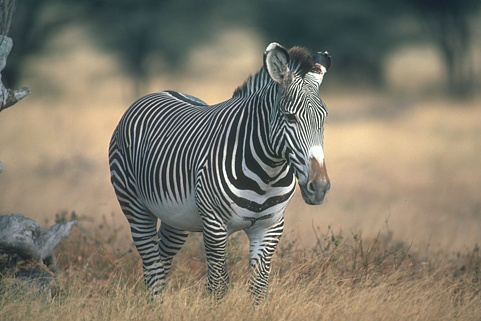
\includegraphics[width=\textwidth]{130066}
    \end{subfigure}
    ~ %add desired spacing between images, e. g. ~, \quad, \qquad, \hfill etc. 
      %(or a blank line to force the subfigure onto a new line)
    \begin{subfigure}[b]{0.2\textwidth}
        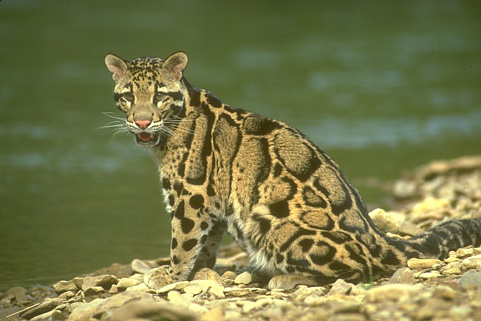
\includegraphics[width=\textwidth]{160067}
    \end{subfigure} \\[2ex]       
    
    \begin{subfigure}[t]{\dimexpr0.2\textwidth+20pt\relax}
    	\makebox[20pt]{\raisebox{25pt}{ \rotatebox[origin=c]{90} {\small \textsf{\textbf{150 sp}}} }}%
    	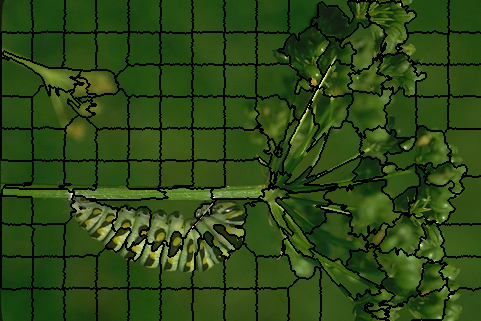
\includegraphics[width=\dimexpr\linewidth-20pt\relax]{35028_wt_150_segs} 
    \end{subfigure}      
    ~ %add desired spacing between images, e. g. ~, \quad, \qquad, \hfill etc. 
      %(or a blank line to force the subfigure onto a new line)
    \begin{subfigure}[b]{0.2\textwidth}
        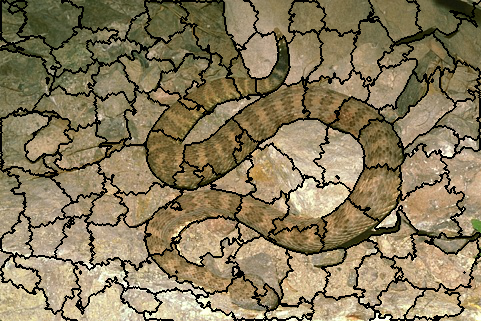
\includegraphics[width=\textwidth]{87015_wt_150_segs}
    \end{subfigure}
    ~ %add desired spacing between images, e. g. ~, \quad, \qquad, \hfill etc. 
      %(or a blank line to force the subfigure onto a new line)
    \begin{subfigure}[b]{0.2\textwidth}
        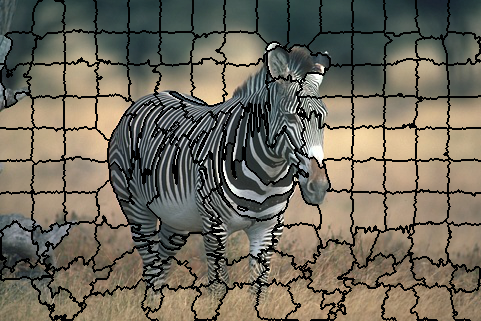
\includegraphics[width=\textwidth]{130066_wt_150_segs}
    \end{subfigure}
    ~ %add desired spacing between images, e. g. ~, \quad, \qquad, \hfill etc. 
      %(or a blank line to force the subfigure onto a new line)
    \begin{subfigure}[b]{0.2\textwidth}
        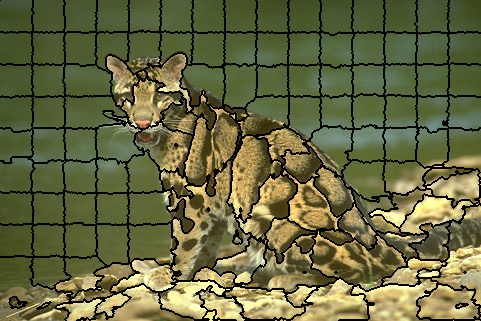
\includegraphics[width=\textwidth]{160067_wt_150_segs}
    \end{subfigure} \\ [2ex]
    
    \begin{subfigure}[t]{\dimexpr0.2\textwidth+20pt\relax}
    	\makebox[20pt]{\raisebox{25pt}{ \rotatebox[origin=c]{90} {\small \textsf{\textbf{300 sp}}} }}%
    	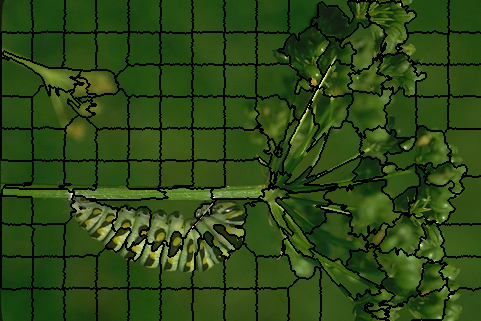
\includegraphics[width=\dimexpr\linewidth-20pt\relax]{35028_wt_150_segs} 
    \end{subfigure}      
    ~ %add desired spacing between images, e. g. ~, \quad, \qquad, \hfill etc. 
      %(or a blank line to force the subfigure onto a new line)
    \begin{subfigure}[b]{0.2\textwidth}
        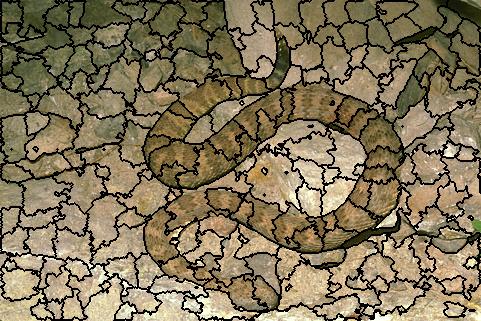
\includegraphics[width=\textwidth]{87015_wt_300_segs}
    \end{subfigure}
    ~ %add desired spacing between images, e. g. ~, \quad, \qquad, \hfill etc. 
      %(or a blank line to force the subfigure onto a new line)
    \begin{subfigure}[b]{0.2\textwidth}
        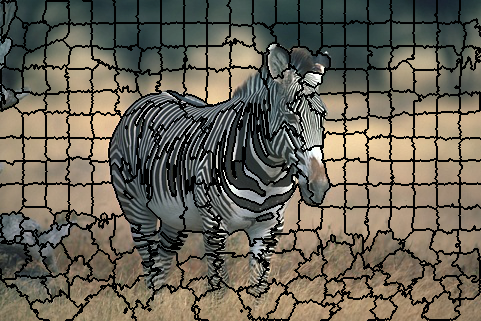
\includegraphics[width=\textwidth]{130066_wt_300_segs}
    \end{subfigure}
    ~ %add desired spacing between images, e. g. ~, \quad, \qquad, \hfill etc. 
      %(or a blank line to force the subfigure onto a new line)
    \begin{subfigure}[b]{0.2\textwidth}
        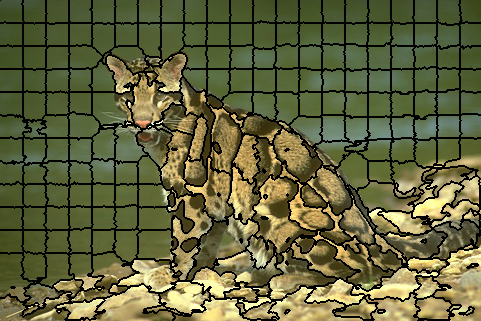
\includegraphics[width=\textwidth]{160067_wt_300_segs}
    \end{subfigure} \\ [2ex]
    
    \begin{subfigure}[t]{\dimexpr0.2\textwidth+20pt\relax}
    	\makebox[20pt]{\raisebox{25pt}{ \rotatebox[origin=c]{90} {\small \textsf{\textbf{600 sp}}} }}%
    	\includegraphics[width=\dimexpr\linewidth-20pt\relax]{35028_wt_600_segs} 
    \end{subfigure}      
    ~ %add desired spacing between images, e. g. ~, \quad, \qquad, \hfill etc. 
      %(or a blank line to force the subfigure onto a new line)
    \begin{subfigure}[b]{0.2\textwidth}
        \includegraphics[width=\textwidth]{87015_wt_600_segs}
    \end{subfigure}
    ~ %add desired spacing between images, e. g. ~, \quad, \qquad, \hfill etc. 
      %(or a blank line to force the subfigure onto a new line)
    \begin{subfigure}[b]{0.2\textwidth}
        \includegraphics[width=\textwidth]{130066_wt_600_segs}
    \end{subfigure}
    ~ %add desired spacing between images, e. g. ~, \quad, \qquad, \hfill etc. 
      %(or a blank line to force the subfigure onto a new line)
    \begin{subfigure}[b]{0.2\textwidth}
        \includegraphics[width=\textwidth]{160067_wt_600_segs}
    \end{subfigure}     

	\caption{Examples of superpixels obtained with the Compact Watershed algorithm.}\label{fig:wt_suprepixels}    
\end{figure}


\subsubsection{SLIC superpixels}
The Simple Linear Iterative Clustering (SLIC) algorithm is part of the superpixel clustering-based methods. The methods in this category group pixels into clusters (superpixels) and iteratively refine such clusters until some convergence criterion is met. In the case of the SLIC, the centers of the clusters are randomly initialized and then associate each pixel to the closest central pixel. The central clusters are subsequently adjusted iteratively until the error converges.

The SLIC algorithm allows controlling (approximately) the number of superpixels in the image, the compactness of the superpixels, and the adherence to the objects' boundaries. However, this method cannot capture the global properties of the image \citep{Stutz.Hermans.ea:CVIU:2018}. Figure \ref{fig:slic_suprepixels} shows, shows, in the same way as the previous algorithms, the method's results demanding 150, 300, and 600 superpixels.


\begin{figure}[!ht]
    \centering
    \begin{subfigure}[t]{\dimexpr0.2\textwidth+20pt\relax}
    	\makebox[20pt]{\raisebox{25pt}{ \rotatebox[origin=c]{90} {\small \textsf{\textbf{Input image}}} }}%
    	\includegraphics[width=\dimexpr\linewidth-20pt\relax]{35028} 
    \end{subfigure}      
    ~ %add desired spacing between images, e. g. ~, \quad, \qquad, \hfill etc. 
      %(or a blank line to force the subfigure onto a new line)
    \begin{subfigure}[b]{0.2\textwidth}
        \includegraphics[width=\textwidth]{87015}
    \end{subfigure}
    ~ %add desired spacing between images, e. g. ~, \quad, \qquad, \hfill etc. 
      %(or a blank line to force the subfigure onto a new line)
    \begin{subfigure}[b]{0.2\textwidth}
        \includegraphics[width=\textwidth]{130066}
    \end{subfigure}
    ~ %add desired spacing between images, e. g. ~, \quad, \qquad, \hfill etc. 
      %(or a blank line to force the subfigure onto a new line)
    \begin{subfigure}[b]{0.2\textwidth}
        \includegraphics[width=\textwidth]{160067}
    \end{subfigure} \\[2ex]       
    
    \begin{subfigure}[t]{\dimexpr0.2\textwidth+20pt\relax}
    	\makebox[20pt]{\raisebox{25pt}{ \rotatebox[origin=c]{90} {\small \textsf{\textbf{150 sp}}} }}%
    	\includegraphics[width=\dimexpr\linewidth-20pt\relax]{35028_slic_150_segs} 
    \end{subfigure}      
    ~ %add desired spacing between images, e. g. ~, \quad, \qquad, \hfill etc. 
      %(or a blank line to force the subfigure onto a new line)
    \begin{subfigure}[b]{0.2\textwidth}
        \includegraphics[width=\textwidth]{87015_slic_150_segs}
    \end{subfigure}
    ~ %add desired spacing between images, e. g. ~, \quad, \qquad, \hfill etc. 
      %(or a blank line to force the subfigure onto a new line)
    \begin{subfigure}[b]{0.2\textwidth}
        \includegraphics[width=\textwidth]{130066_slic_150_segs}
    \end{subfigure}
    ~ %add desired spacing between images, e. g. ~, \quad, \qquad, \hfill etc. 
      %(or a blank line to force the subfigure onto a new line)
    \begin{subfigure}[b]{0.2\textwidth}
        \includegraphics[width=\textwidth]{160067_slic_150_segs}
    \end{subfigure} \\ [2ex]
    
    \begin{subfigure}[t]{\dimexpr0.2\textwidth+20pt\relax}
    	\makebox[20pt]{\raisebox{25pt}{ \rotatebox[origin=c]{90} {\small \textsf{\textbf{300 sp}}} }}%
    	\includegraphics[width=\dimexpr\linewidth-20pt\relax]{35028_slic_150_segs} 
    \end{subfigure}      
    ~ %add desired spacing between images, e. g. ~, \quad, \qquad, \hfill etc. 
      %(or a blank line to force the subfigure onto a new line)
    \begin{subfigure}[b]{0.2\textwidth}
        \includegraphics[width=\textwidth]{87015_slic_300_segs}
    \end{subfigure}
    ~ %add desired spacing between images, e. g. ~, \quad, \qquad, \hfill etc. 
      %(or a blank line to force the subfigure onto a new line)
    \begin{subfigure}[b]{0.2\textwidth}
        \includegraphics[width=\textwidth]{130066_slic_300_segs}
    \end{subfigure}
    ~ %add desired spacing between images, e. g. ~, \quad, \qquad, \hfill etc. 
      %(or a blank line to force the subfigure onto a new line)
    \begin{subfigure}[b]{0.2\textwidth}
        \includegraphics[width=\textwidth]{160067_slic_300_segs}
    \end{subfigure} \\ [2ex]       
    
    \begin{subfigure}[t]{\dimexpr0.2\textwidth+20pt\relax}
    	\makebox[20pt]{\raisebox{25pt}{ \rotatebox[origin=c]{90} {\small \textsf{\textbf{600 sp}}} }}%
    	\includegraphics[width=\dimexpr\linewidth-20pt\relax]{35028_slic_600_segs} 
    \end{subfigure}      
    ~ %add desired spacing between images, e. g. ~, \quad, \qquad, \hfill etc. 
      %(or a blank line to force the subfigure onto a new line)
    \begin{subfigure}[b]{0.2\textwidth}
        \includegraphics[width=\textwidth]{87015_slic_600_segs}
    \end{subfigure}
    ~ %add desired spacing between images, e. g. ~, \quad, \qquad, \hfill etc. 
      %(or a blank line to force the subfigure onto a new line)
    \begin{subfigure}[b]{0.2\textwidth}
        \includegraphics[width=\textwidth]{130066_slic_600_segs}
    \end{subfigure}
    ~ %add desired spacing between images, e. g. ~, \quad, \qquad, \hfill etc. 
      %(or a blank line to force the subfigure onto a new line)
    \begin{subfigure}[b]{0.2\textwidth}
        \includegraphics[width=\textwidth]{160067_slic_600_segs}
    \end{subfigure}     
    
	\caption{Examples of superpixels generated with SLIC algorithm.}\label{fig:slic_suprepixels}    
\end{figure}

In this work, we choose the SLIC algorithm to generate the superpixels of the images. This method is one of the most competent in terms of customization and calculation time. Furthermore, it is possible to use the image in the LAB color space to form superpixels according to the image's perceptual colors. For more details on the implementation and performance of the different superpixel algorithms, we invite the reader to review the work of \cite{Wang.Liu.ea:SP:2017}.

\section{Graph-based Image Gradient and Segmentation}

In this section, we develop the methodology to obtain a perceptual gradient on an image-graph. Such an image gradient is said perceptual as it is based on the multispectral decomposition of an image using Gabor filters. We use EMD as a measure of similarity between the graph's nodes to define the edges' weight. Specifications and adaptations of the EMD are also developed in this section. Subsequently, we use the resulting gradients to segment the image using well-known state-of-the-art techniques.  

\subsection{Earth Mover's Distance for Non-normalized Distributions}
In chapter \ref{ch:similarity_measures}, we have seen the utility of the EMDas a true metric for measuring similarity between distributions. In image retrieval systems based on color information, the EMD can measure tiny changes in the normalized color distributions of superhero images. On the other hand, with the texture patches, the EMD can capture, reflect and measure the importance of the logarithmic (frequency) and polar (orientation) axis of the texture signature (see figure \ref{fig:MDS_EMD} in section \ref{ch:suplementary_material_retrieval_systems}). This chapter uses EMD to measure the similarity between two elements of an image: pixels or superpixels. By measuring the similarity of elements in Gabor's feature space, we locally measure changes in color and texture in the image. 

The EMD \citep{Rubner.Tomasi.ea:IJCV:2000} , as we used it to measure color and texture distributions in chapter \ref{ch:similarity_measures} (cf. Eq. \eqref{eq:emd}), is a true metric only when used with normalized distributions (histograms or signatures), i.e., distributions with total mass equal to one. This fact has no impact when the distributions represent global information of an image (color or texture). However, the distributions of the image elements (pixels or superpixels) contain only a portion of the information; for example, in the case of our feature space, Gabor's energy. 

Normalizing the individual pixels or superpixels' texture signatures leads to Gabor energy information loss, so the classic EMD cannot be applied. We use instead the EMD proposed by \citep{Pele.Werman::2008}.

\begin{eqnarray}
d_{\widehat{EMD}}(P, Q) = \left( \underset{\{f_{ij}\}}{\mathrm{min}}\sum_{i,j}f_{ij}c_{ij}\right)
+ \left\vert \sum_{i} P_i - \sum_{j} Q_j \right\vert \times \alpha\, \underset{{i,j}}{\mathrm{max}} \{c_{ij}\}  \quad \text{s.t.}\nonumber \label{eq:emd_pele} \\
\sum_{j}f_{ij} \leq P_i \, , \; \sum_{i}f_{ij} \leq Q_j \, , \; \sum_{i,j}f_{ij} \leq Q_j \, , \; \sum_{i,j}f_{ij} = \mathrm{min} \left( \sum_{i} P_i , \sum_{j} Q_j\right)\, , \; f_{ij} \geq 0
\end{eqnarray}
where $f_{ij}$ denotes the amount transported and $c_{ij}$ denotes the transport cost from the $i$th supplier in $P$ to the $j$th consumer in $Q$. 

\subsection{Graph Image Gradients}
As we described earlier, we can use pixels or superpixels as support to represent an image as a graph. Figure \ref{fig:computational_support} shows a natural-color image, its superpixels obtained with the SLIC technique (approximately 2500 regions), and the region adjacency graph obtained on the superpixels. In this sense, each node of the graph is positioned at the centroid of each superpixel in the image. This strategy allows reducing the EMD calculation time between nodes of the graph, with the compromise. The pixel adjacency graph of the image is not displayed (see instead \ref{fig:pag_example} as a PAG reference); however, we used a 4 neighboring node adjacency system (4nn) for its creation.

\begin{figure}[!ht]
    \centering
    \begin{subfigure}[b]{0.49\textwidth}
    	\includegraphics[width=\textwidth]{100007} 
    	\caption{Input image}
    \end{subfigure}    
    \begin{subfigure}[b]{0.49\textwidth}
        \includegraphics[width=\textwidth]{100007_slic}
        \caption{SLIC superpixels}
    \end{subfigure}\\    
    \begin{subfigure}[b]{0.49\textwidth}
        \includegraphics[width=\textwidth]{100007_raw_rag}
        \caption{Unweighted superpixel RAG}
    \end{subfigure}
    
	\caption{Computational support for graph-based image gradient.}\label{fig:computational_support}    
\end{figure}

The weight of the edges between nodes of both computational supports is given by the EMD for non-normalized distributions. 
\begin{equation}
	\mathsf{e}_{ij} \leftarrow \omega(\mathsf{v}_i, \mathsf{v}_j) = d_{\widehat{EMD}}(\widetilde{e}(i), \widetilde{e}(j))
\end{equation}
In color images, we obtain a weighted edge graph for each channel of the complex luminance-chrominance color space. Figure \ref{fig:graph_gradient_pixel_superpixel} shows the weighted graphs of each channel of a natural image based on pixels and superpixels. 

\begin{figure}[!ht]
    \centering
    \begin{subfigure}[b]{0.49\textwidth}
    	\includegraphics[width=\textwidth]{100007_lum_grad} 
    \end{subfigure}         
    \begin{subfigure}[b]{0.49\textwidth}
        \includegraphics[width=\textwidth]{100007_weighted_lum_rag}
    \end{subfigure}\\ [1ex]    
    \begin{subfigure}[b]{0.49\textwidth}
        \includegraphics[width=\textwidth]{100007_cr_grad}
    \end{subfigure}     
    \begin{subfigure}[b]{0.49\textwidth}
    	\includegraphics[width=\textwidth]{100007_weighted_cr_rag} 
    \end{subfigure}\\ [1ex]          
    \begin{subfigure}[b]{0.49\textwidth}
        \includegraphics[width=\textwidth]{100007_ci_grad}
        \caption{Pixel-based graph gradient}
    \end{subfigure}   
    \begin{subfigure}[b]{0.49\textwidth}
        \includegraphics[width=\textwidth]{100007_weighted_ci_rag}
        \caption{Region-based graph gradient}
    \end{subfigure}
    
	\caption{Graph gradient images. First row: Luminance channel, second raw: Chrominance (real part), and third raw: Chrominance (imag part). The raws names indicate the respective graph structure used to compute the gradient.}\label{fig:graph_gradient_pixel_superpixel}    
\end{figure}

The gradients obtained with this methodology follow the color and texture variations of the authentic images. Furthermore, an essential aspect of our methodology is that the image's decomposition using the optimized Gabor filters and the complex color space respects Parseval's identity. In other words, the sum of all Gabor responses (in frequency axis, angular axis, and per color channel) is equal to 1. This property is reflected in the weights of the edges of the luminance and chrominance graphs. Generally, the luminance channel is the one that recovers most of the energy, while the color energy is divided into the real and imaginary parts of the chrominance. In the gradients of the second row of images of figure \ref{fig:graph_gradient_pixel_superpixel}, the maximum distance between two nodes in the luminance channel is approximately 30, while in the real and imaginary part of the chrominance, the distance varies between 10 and 14. This property allows us to add the weights of the edges of each channel's graphs to obtain a single graph gradient. We can see the total gradients in the pixel and superpixel support in figure \ref{fig:total_graph_gradient_pixel_superpixel}.

\begin{figure}[!ht]
    \centering
    \begin{subfigure}[b]{0.49\textwidth}
    	\includegraphics[width=\textwidth]{100007_pred_grad} 
    \end{subfigure}      
    %add desired spacing between images, e. g. ~, \quad, \qquad, \hfill etc. 
      %(or a blank line to force the subfigure onto a new line)
    \begin{subfigure}[b]{0.49\textwidth}
        \includegraphics[width=\textwidth]{100007_weighted_pred}
    \end{subfigure}    
	\caption{Total graph gradient images.}\label{fig:total_graph_gradient_pixel_superpixel}    
\end{figure}

\subsection{Image Segmentation Based on Image Gradients}
The perceptual gradients obtained with EMD contain the necessary structure to segment images using graph-based segmentation methods. We use the adjacency matrix of the graph for this purpose. Here we present the methodology and results of three different segmentation methods on the weighted graphs on the superpixel support; pixel-level graphs are not considered due to the high computation time. 

\subsubsection{MST threshold graph-cut}

This image segmentation method consists of obtaining the minimum spanning tree (MTS) of the total edge-weighted graph (with normalized values between 0 and 1) and then perform a cut over the graph. Since in the MST, there is only a single path that joins all the nodes of the graph, we can make one or more graph cuts to separate the image into regions. We define the edges that are removed by the cut setting a threshold value over the weights of the MST edges. This threshold value choice is not always obvious, and this value may differ for each image.

We propose obtaining a threshold value by fitting a probability density function to the distribution of the MST edges values. We hypothesize that the areas with the same color and (or) texture information behave as flat areas in the generated feature space; therefore, the edges that connect these areas have a considerable EMD value and behave as outliers within the probability function. We choose the logarithmic distribution as the density function to fit. The threshold value is defined then by the log distribution point where the edge weights reach the quantile of order $q = 0.9$. Under this setting, we cut all the MST edges above the quantile and keep $90\%$ of the graph's edges. The segmentation of the image is given by the connected components of the resulting graph.

Taking the example of the polar bear image, figure \ref{fig:graphcut_segmentation_technique}  shows the MST graph of the image and the weight distribution of the MST edges (black bars), and the logarithmic distribution (red line) that matches the weight histogram. The red arrow on the plot shows the threshold value for cutting the graph. The resulting segmentation is shown in subfigure \ref{fig:graphcut_segmentation_result}.

\begin{figure}[!ht]
    \centering
    \begin{subfigure}[b]{0.49\textwidth}
    	\includegraphics[width=\textwidth]{100007_weighted_mstgraph}
    	\caption{edge-weighted MTS} 
    \end{subfigure}      
    %add desired spacing between images, e. g. ~, \quad, \qquad, \hfill etc. 
      %(or a blank line to force the subfigure onto a new line)
    \begin{subfigure}[b]{0.49\textwidth}
        \includegraphics[width=\textwidth]{100007_weight_dist}
        \caption{MTS weights distribution}
    \end{subfigure}\\ [1ex]
    %add desired spacing between images, e. g. ~, \quad, \qquad, \hfill etc. 
      %(or a blank line to force the subfigure onto a new line)
    \begin{subfigure}[b]{0.49\textwidth}
        \includegraphics[width=\textwidth]{100007_graphcut_result}
        \caption{Threshold graph-cut segmentation result}
        \label{fig:graphcut_segmentation_result}
    \end{subfigure}    
    
	\caption{Stages of threshold graph-cut segmentation technique.}\label{fig:graphcut_segmentation_technique}    
\end{figure}

An advantage of this method is the computational speed to obtain an image segmentation. Furthermore, selecting the threshold value for the graph cut is independent of the user and self-adapting for each image. However, the choice of the quantile $q$ is important; a very low value leads to cutting edges within flat areas of color and (or) texture, generating an over-segmentation of the image; on the other hand, a high threshold value leads to preserving most of the edges so that most of the image regions remain connected.

\subsubsection{Spectral clustering}

The spectral clustering is a technique used to cluster elements of a graph \citep{Ng.Jordan.ea:NIPS:2001}. Considering the RAG weighted with the EMD over the Gabor feature space, we used this technique to group the superpixels into perceptual regions consistent with the color and texture information.

This technique transfers the data from a given domain to the spectral domain using eigendecomposition. The general process of spectral clustering is mainly divided into the following three stages:

\begin{itemize}
	\item Preprocessing: Construct a similarity matrix.
	\item Decomposition: Compute the Laplacian graph's eigenvectors to embed the data points in a low-dimensional space (spectral embedding).
	\item Grouping: Assign the points in k clusters based on the new representation using the k-means algorithm.
\end{itemize}

Detailing the stages of spectral clustering, we obtain the affinity matrix $A = (A_{ij})$ from the graph based on superpixels. The elements of the matrix are given by the function
\begin{equation}	
	A_{ij}= 
	\begin{cases}
		\exp{\left(- \alpha \frac{\omega_{ij}}{\sigma(W)}\right)}  \quad \text{if $i, j$ are adjacent in $\mathcal{G}$} \\
		0 \quad \text{elsewhere}
	\end{cases}	 
\end{equation}
where $\omega_{ij}$ is the measure of distance between nodes of the graph (given by the EMD between non-normalized distributions); $\sigma(W)$ is the total standard deviation of the weight matrix $W$ that serves a global optimization parameter for the affinity matrix computation and; $\alpha$ is a human-defined constant which controls how rapidly the affinity $A_{ij}$ falls off with the distance between $i$ and $j$.

The spectral decomposition is done using the Laplacian matrix, which depends on the affinity matrix $A$ and the matrix of degree $D$. We follow the algorithm of \cite{Ng.Jordan.ea:NIPS:2001}, which proposes to use the normalized Laplacian matrix $L = D^{-1/2} A D^{-1/2}$. This Laplacian matrix form is known as the non-normalized one. Once the k largest eigenvectors of $ L $ have been found and normalized, we apply the k-means algorithm on the data points of this reduced space of the graph and assign each node to a cluster.

Figure \ref{fig:spectral_clustering_process} shows the similarity graph constructed from the EMD distances between texture signatures. Since the similarity function $s(i, j)$ is inverse to the distance $\omega (i, j)$ between nodes, we see that the edges' value tends to $0$ (black edges) when the regions are dissimilar, and when the regions are similar, the edges' value tends to $1$ (white edges). Subfigure \ref{fig:spectral_clustering_segm_result} shows the polar bear segmentation result using $k = \mathrm{min}(\mathcal{S})$ (which for this image $k =5$) and $\alpha = 6$.

\begin{figure}[!ht]
    \centering
    \begin{subfigure}[b]{0.49\textwidth}
    	\includegraphics[width=\textwidth]{100007_weighted_completegraph} 
    	\caption{Affinity graph}
    \end{subfigure}      
    %add desired spacing between images, e. g. ~, \quad, \qquad, \hfill etc. 
      %(or a blank line to force the subfigure onto a new line)
    \begin{subfigure}[b]{0.49\textwidth}
        \includegraphics[width=\textwidth]{100007_spec_result}
        \caption{Spectral clustering segmentation result}
        \label{fig:spectral_clustering_segm_result} 
    \end{subfigure}    
	\caption{Gradient-based spectral clustering segmentation.}\label{fig:spectral_clustering_process}    
\end{figure}


\subsubsection{Normalized graph-cut}
The Normalized cuts technique is a variation of the spectral clustering technique to cluster graphs. Initially proposed by \cite{JianboShi.Malik:PAMI:2000}, this method performs the same spectral clustering steps described above with some minor differences. As for the affinity matrix, it remains the same. However, the Laplacian matrix here is given as
$L_{Ncut} = D^{-1}L$
so the eigendecomposition problem is different as well.

Furthermore, the normalized cut is a recursive method that finds a bipartition of the graph to maximize $Ncut$. This process is repeated considering the stability of the cut and if $Ncut$ is below the preset value. This condition implies that, unlike spectral clustering, we do not need to introduce a specific number of regions $k$ to find in the image. We find more details about this method in \cite{JianboShi.Malik:PAMI:2000}. We show the segmentation result of the polar bear image using the normalized cut method in figure \ref{fig:norm_cut_segm_result}. 

\begin{figure}[!ht]
    \centering
  	\includegraphics[width=0.49\textwidth]{100007_ncut_result}
    \caption{Normalized cut segmentation result.}
    \label{fig:norm_cut_segm_result}    
\end{figure}


\subsubsection{Comparison of the Different Graph-based Segmentation Methods}
We evaluate the quality of the segmentation given by the three segmentation methods based on graphs: MST threshold graph-cut, Spectral clustering, and Normalized graph-cut.  For this, we use the Berkeley image database test set and the F-measure obtained from the precision and recall scores described in chapter \ref{ch:complex_spectral_image_decomposition}. 

In figure \ref{fig:boxplot_score_methods}, we show the resulting scores applying the segmentation methods to graphs built in different feature spaces. In particular, we vary the input color space to construct the luminance-chrominance representation of the image.

\begin{figure}[!ht]
    \centering
    \begin{subfigure}[b]{0.49\textwidth}
        \includegraphics[width=\textwidth]{Thr_graphcut_scores_log_mst_boxplot}
        \caption{Threshold graph-cut}
    \end{subfigure}     
    \begin{subfigure}[b]{0.49\textwidth}
    	\centering
    	\includegraphics[width=\textwidth]{Spectral_clustering_scores_global_complete_boxplot}
        \caption{Spectral clustering}
    \end{subfigure}     
    \begin{subfigure}[b]{0.49\textwidth}
    	\centering
        \includegraphics[width=\textwidth]{Normalized_graphcut_scores_global_complete_boxplot}
        \caption{Normalized graph-cut}
    \end{subfigure} 
        	    
    \caption{Segmentation scores of the different graph-based segmentation methods.}\label{fig:boxplot_score_methods}    
\end{figure}

\section{Image Contour Detection and Segmentation}

The graph-based segmentation methods presented above showed exciting results in the segmentation task of natural color images. However, these methods require a series of parameters that are often not so easy to define, for example, the number of $k$ regions to segment, the $\alpha$ parameter for constructing the affinity matrix, and the stop point of the normalized cut algorithm. Although there are various literature methods to optimize and automate the choice of such parameters, this implies a longer calculation time to obtain a segmentation. The peculiarity of these methods is that they depend on an over-segmentation in superpixels before calculating the graph's gradient. Although this step reduces the number of nodes and, consequently, the number of edges and EMD to be calculated, the contours in the image's final segmentation are part of the superpixel method's contours. In other words, if the boundaries of the regions thrown by the SLIC algorithm do not correspond to the contours of the objects in the images, these borders will not appear in the final segmentation. 

This section presents the methodology to obtain the objects' perceptual contours in an image directly using the information from the edge-weighted graph instead of using graph-based segmentation methods. The main advantage of this approach is that the image's contours can be obtained at the pixel and superpixel levels. The procedure for obtaining the contours is straightforward. The similarity between the image elements (pixels or superpixels) is calculated by the EMD and stored in the graph's edges. So, in the case of a graph at a pixel level, the perceptual contours are obtained with the transformation of the edge-weighted graph into a node-weighted graph, where the value of each node (pixel) is the maximum value between the weights of all the edges connected to the node. In the case of superpixels, we transform the edge-weighted graph into a perceptual contour image by assigning the weight of the edge between two regions to the pixels that form the common border between these superpixels. Figure \ref{fig:GCC_results} shows some examples of the contours found with this methodology in images of the BSDS500 using the graphs at the pixel and superpixel levels. 

\begin{figure}[!ht] 
   
    \begin{subfigure}[t]{\dimexpr0.23\textwidth+20pt\relax}
    	\centering
    	\makebox[20pt]{\raisebox{30pt}{ \rotatebox[origin=c]{90} {\small \textsf{\textbf{Input image}}} }}%
    	\includegraphics[width=\dimexpr\linewidth-20pt\relax]{175083} 
    \end{subfigure}      
%    ~ %add desired spacing between images, e. g. ~, \quad, \qquad, \hfill etc. 
%      %(or a blank line to force the subfigure onto a new line)
    \begin{subfigure}[b]{0.23\textwidth}
    	\centering
        \includegraphics[height=67.68857pt]{101084}
    \end{subfigure}
%    ~ %add desired spacing between images, e. g. ~, \quad, \qquad, \hfill etc. 
%      %(or a blank line to force the subfigure onto a new line)
    \begin{subfigure}[b]{0.23\textwidth}
    	\centering
        \includegraphics[height=67.68857pt]{41096}
    \end{subfigure}
%    ~ %add desired spacing between images, e. g. ~, \quad, \qquad, \hfill etc. 
%      %(or a blank line to force the subfigure onto a new line)
    \begin{subfigure}[b]{0.23\textwidth}
    	\centering
        \includegraphics[height=67.68857pt]{2018}
    \end{subfigure} \\ \vspace{-5pt}      
    
    \begin{subfigure}[t]{\dimexpr0.23\textwidth+20pt\relax}
    	\centering
    	\makebox[20pt]{\raisebox{30pt}{ \rotatebox[origin=c]{90} {\small \textsf{\textbf{GT}}} }}%
    	\includegraphics[width=\dimexpr\linewidth-20pt\relax]{175083_gt_grad} 
    \end{subfigure}      
%    ~ %add desired spacing between images, e. g. ~, \quad, \qquad, \hfill etc. 
%      %(or a blank line to force the subfigure onto a new line)
    \begin{subfigure}[b]{0.23\textwidth}
    	\centering
        \includegraphics[height=67.68857pt]{101084_gt_grad}
    \end{subfigure}
%    ~ %add desired spacing between images, e. g. ~, \quad, \qquad, \hfill etc. 
%      %(or a blank line to force the subfigure onto a new line)
    \begin{subfigure}[b]{0.23\textwidth}
    	\centering
        \includegraphics[height=67.68857pt]{41096_gt_grad}
    \end{subfigure}
%    ~ %add desired spacing between images, e. g. ~, \quad, \qquad, \hfill etc. 
%      %(or a blank line to force the subfigure onto a new line)
    \begin{subfigure}[b]{0.23\textwidth}
    	\centering
        \includegraphics[height=67.68857pt]{2018_gt_grad}
    \end{subfigure} \\ \vspace{-5pt}   
    
    \begin{subfigure}[t]{\dimexpr0.23\textwidth+20pt\relax}
    	\centering
    	\makebox[20pt]{\raisebox{30pt}{ \rotatebox[origin=c]{90} {\small \textsf{\textbf{4nn}}} }}%
    	\includegraphics[width=\dimexpr\linewidth-20pt\relax]{175083_4nn_cont} 
    \end{subfigure}      
%    ~ %add desired spacing between images, e. g. ~, \quad, \qquad, \hfill etc. 
%      %(or a blank line to force the subfigure onto a new line)
    \begin{subfigure}[b]{0.23\textwidth}
    	\centering
        \includegraphics[height=67.68857pt]{101084_4nn_cont}
    \end{subfigure}
%    ~ %add desired spacing between images, e. g. ~, \quad, \qquad, \hfill etc. 
%      %(or a blank line to force the subfigure onto a new line)
    \begin{subfigure}[b]{0.23\textwidth}
    	\centering
        \includegraphics[height=67.68857pt]{41096_4nn_cont}
    \end{subfigure}
%    ~ %add desired spacing between images, e. g. ~, \quad, \qquad, \hfill etc. 
%      %(or a blank line to force the subfigure onto a new line)
    \begin{subfigure}[b]{0.23\textwidth}
    	\centering
        \includegraphics[height=67.68857pt]{2018_4nn_cont}
    \end{subfigure} \\ \vspace{-5pt} 
    
    \begin{subfigure}[t]{\dimexpr0.23\textwidth+20pt\relax}
    	\centering
    	\makebox[20pt]{\raisebox{30pt}{ \rotatebox[origin=c]{90} {\small \textsf{\textbf{2500}}} }}%
    	\includegraphics[width=\dimexpr\linewidth-20pt\relax]{175083_2500sp_cont} 
    \end{subfigure}      
%    ~ %add desired spacing between images, e. g. ~, \quad, \qquad, \hfill etc. 
%      %(or a blank line to force the subfigure onto a new line)
    \begin{subfigure}[b]{0.23\textwidth}
    	\centering
        \includegraphics[height=67.68857pt]{101084_2500sp_cont}
    \end{subfigure}
%    ~ %add desired spacing between images, e. g. ~, \quad, \qquad, \hfill etc. 
%      %(or a blank line to force the subfigure onto a new line)
    \begin{subfigure}[b]{0.23\textwidth}
    	\centering
        \includegraphics[height=67.68857pt]{41096_2500sp_cont}
    \end{subfigure}
%    ~ %add desired spacing between images, e. g. ~, \quad, \qquad, \hfill etc. 
%      %(or a blank line to force the subfigure onto a new line)
    \begin{subfigure}[b]{0.23\textwidth}
    	\centering
        \includegraphics[height=67.68857pt]{2018_2500sp_cont}
    \end{subfigure}   
    
	\caption{Some examples of image contours obtained with the Gabor Complex Color (GCC) feature space on the support of pixels (4nn) and superpixels (2500) graph.}\label{fig:GCC_results}    
\end{figure}


\subsection{Contour-based Image Segmentation: Hierarchical Watershed}

Image segmentation is a complementary problem to contour detection. Some methods, such as the UCM \citep{Arbelaez.Maire.ea:PR:2009}, generate a hierarchical partition of the image from an image contours. In a partition hierarchy, the image is represented as a sequence of coarse to fine partitions that satisfy the principle of causality of \cite{Koenderink:BC:1984}, that is, any partition is a refinement of the previous one in the sequence \citep{Perret.Cousty.ea:TIP:2018}.

We only use the gradient information resulting from the edge-weighted graph's transformation to a boundary image (described in the previous section) in a classic morphological approach for image segmentation, the so-called watershed. This approach complies with the principle of causality, so defining a hierarchy of watersheds as a sequence of watershed segmentation of an image is possible. 

One of the first authors to study the properties and relationship between the partition hierarchy and the watershed operator for image segmentation are \citep{Najman.Schmitt:PAMI:1996}. In general terms, this method constructs a watershed by a flooding process; that is, the gradient image, seen as a topographic surface, is pierced at its minima and progressively submerged in water. The water fills the catchment basins of the minima and forms lakes. When the water of two lakes meets, the saddle point height where this occurs determines the saliency of the corresponding watershed arch. The sequence of watershed segmentation is obtained by sequentially removing the minima from the gradient image according to regional attributes related to size and the contrast of the components, such as dynamics, area, or volume. In figure \ref{fig:GCC_higra_results}, we show the results of hierarchical watershed segmentation using the volume attribute on the GCC4nn and GCC2500 image gradients. 

\begin{figure}[!ht] 
   
    \begin{subfigure}[t]{\dimexpr0.23\textwidth+20pt\relax}
    	\centering
    	\makebox[20pt]{\raisebox{30pt}{ \rotatebox[origin=c]{90} {\small \textsf{\textbf{Input image}}} }}%
    	\includegraphics[width=\dimexpr\linewidth-20pt\relax]{175083} 
    \end{subfigure}      
%    ~ %add desired spacing between images, e. g. ~, \quad, \qquad, \hfill etc. 
%      %(or a blank line to force the subfigure onto a new line)
    \begin{subfigure}[b]{0.23\textwidth}
    	\centering
        \includegraphics[height=67.68857pt]{101084}
    \end{subfigure}
%    ~ %add desired spacing between images, e. g. ~, \quad, \qquad, \hfill etc. 
%      %(or a blank line to force the subfigure onto a new line)
    \begin{subfigure}[b]{0.23\textwidth}
    	\centering
        \includegraphics[height=67.68857pt]{41096}
    \end{subfigure}
%    ~ %add desired spacing between images, e. g. ~, \quad, \qquad, \hfill etc. 
%      %(or a blank line to force the subfigure onto a new line)
    \begin{subfigure}[b]{0.23\textwidth}
    	\centering
        \includegraphics[height=67.68857pt]{2018}
    \end{subfigure} \\ \vspace{-5pt}      
    
        
    \begin{subfigure}[t]{\dimexpr0.23\textwidth+20pt\relax}
    	\centering
    	\makebox[20pt]{\raisebox{30pt}{ \rotatebox[origin=c]{90} {\small \textsf{\textbf{4nn}}} }}%
    	\includegraphics[width=\dimexpr\linewidth-20pt\relax]{175083_4nn_higra} 
    \end{subfigure}      
%    ~ %add desired spacing between images, e. g. ~, \quad, \qquad, \hfill etc. 
%      %(or a blank line to force the subfigure onto a new line)
    \begin{subfigure}[b]{0.23\textwidth}
    	\centering
        \includegraphics[height=67.68857pt]{101084_4nn_higra}
    \end{subfigure}
%    ~ %add desired spacing between images, e. g. ~, \quad, \qquad, \hfill etc. 
%      %(or a blank line to force the subfigure onto a new line)
    \begin{subfigure}[b]{0.23\textwidth}
    	\centering
        \includegraphics[height=67.68857pt]{41096_4nn_higra}
    \end{subfigure}
%    ~ %add desired spacing between images, e. g. ~, \quad, \qquad, \hfill etc. 
%      %(or a blank line to force the subfigure onto a new line)
    \begin{subfigure}[b]{0.23\textwidth}
    	\centering
        \includegraphics[height=67.68857pt]{2018_4nn_higra}
    \end{subfigure} \\ \vspace{-5pt} 
    
    \begin{subfigure}[t]{\dimexpr0.23\textwidth+20pt\relax}
    	\centering
    	\makebox[20pt]{\raisebox{30pt}{ \rotatebox[origin=c]{90} {\small \textsf{\textbf{2500}}} }}%
    	\includegraphics[width=\dimexpr\linewidth-20pt\relax]{175083_2500sp_higra} 
    \end{subfigure}      
%    ~ %add desired spacing between images, e. g. ~, \quad, \qquad, \hfill etc. 
%      %(or a blank line to force the subfigure onto a new line)
    \begin{subfigure}[b]{0.23\textwidth}
    	\centering
        \includegraphics[height=67.68857pt]{101084_2500sp_higra}
    \end{subfigure}
%    ~ %add desired spacing between images, e. g. ~, \quad, \qquad, \hfill etc. 
%      %(or a blank line to force the subfigure onto a new line)
    \begin{subfigure}[b]{0.23\textwidth}
    	\centering
        \includegraphics[height=67.68857pt]{41096_2500sp_higra}
    \end{subfigure}
%    ~ %add desired spacing between images, e. g. ~, \quad, \qquad, \hfill etc. 
%      %(or a blank line to force the subfigure onto a new line)
    \begin{subfigure}[b]{0.23\textwidth}
    	\centering
        \includegraphics[height=67.68857pt]{2018_2500sp_higra}
    \end{subfigure}   
    
	\caption{Some examples of image segmentations obtained with the hirachical watershed method on the Gabor Complex Color (GCC) boundaries in the pixels level support (4nn) and superpixels (2500) support.}\label{fig:GCC_higra_results}    
\end{figure}
%\subsection{Interactive image segmentation}



\section{Comparison with the State-of-the-Art}
In section \ref{sec:soa_boundaries_segmentation}, we review the different methods for detecting contours and the segmentation of natural images. This section classifies state-of-the-art methods based on the input features and the techniques used for contour detection and image segmentation. Table \ref{table:characteristics_soa_methods} organizes the various characteristics of these methods, which allows us to position our contour detector (GCC) w.r.t. the existing works.

We recall that one of the thesis's objectives is to generate algorithms for the detection of objects in complex environments to implement them in the context of UAV tasks. In this sense, the characteristics that we look for in a contour detector are:

\begin{itemize}
	\item the independence of databases to train learning models,
	\item the simplicity and a low number of parameters, and
	\item the possible real-time implementation.
\end{itemize}    

Taking this into account, table \ref{table:characteristics_soa_methods} separates state-of-the-art methods into three groups: non-supervised (N-S), semi-supervised (S-S), and fully supervised (F-S) approaches. Our contour detector is positioned in the group of non-supervised methods (first column of the table together with the Pb and the PMI methods). 

\begin{table}[!h]
\resizebox{\textwidth}{!}{%
\begin{tabular}{c|c|c|c}
\textbf{Edge detector} & \textbf{Input features}                                                                           & \textbf{Main approach}                                           & \textbf{\begin{tabular}[c]{@{}c@{}}Segmentation \\ technique\end{tabular}} \\ \hline
GCC (Ours)				& Gabor lum-chr gradients																			& Gradients dissimilarity							& Hierarchical Watershed													 \\                                         
Pb                      & BG, TG                                                                                            & Gradients dissimilarity                                          & Normalized cuts                                                            \\
PMI                     & LUV color channels                                                                                & Pixel mutual information                                         & Spectral clustering                                                                          \\ \hline
SCG                     & \begin{tabular}[c]{@{}c@{}}Gray, color, and \\ depth channels\end{tabular}                        & \begin{tabular}[c]{@{}c@{}}Sparse coding\\ +\\ SVM\end{tabular}  & -                                                                          \\
SCT                     & RGB color channels                                                                                & \begin{tabular}[c]{@{}c@{}}Sparse coding\\  +\\ SVM\end{tabular} & -                                                                          \\ \hline
$\widehat{\text{Pb}}$   & BG, TG                                                                                            & Logistic regression                                              & Normalized cuts                                                            \\
gPb                     & $\widehat{\text{OE}}$, BG, CG, $\widehat{\text{TG}}$                                              & Logistic regression                                              & UCM + OWT                                                                  \\
BEL                     & Integral channel features                                                                         & Gradient boosting                                                & -                                                                          \\
Sketch tokens           & Integral channel features                                                                         & Random forest                                                    & -                                                                          \\
SE                      & Integral channel features                                                                         & Random forest                                                    & -                                                                          \\
OEF                     & Integral channel features                                                                         & Random forest                                                    & -                                                                          \\
DeepNet                  & Covariance-like features                                                                          & Deep NN                                                          & -                                                                          \\
ISCRA                   & \begin{tabular}[c]{@{}c@{}}BG, CG, TG, SIFT,\\  shape features, \\ boundary features\end{tabular} & Cascading classifier                                             & Region merging                                                             \\
COB                     & $\widehat{\text{OE}}$, BG, CG, $\widehat{\text{TG}}$                                              & Convolutional NN                                                 & -                                                                       
\end{tabular}}
\caption{Principal characteristics of the state-of-the-art works for boundary detection and image segmentation. First block: Non-supervised methods, Second block: Semi-supervised methods, and Third block: Supervised methods.}
\label{table:characteristics_soa_methods}
\end{table}


\subsection{Scores}
We use the benchmark for contour detection and image segmentation of the BSDS. This benchmark uses the precision and recall scores described in chapter \ref{ch:complex_spectral_image_decomposition} (cf. subsection \ref{subsec:quantitative_evaluation}). In addition to these scores, the BSDS benchmark uses the following measures and tools to compare results in contour detection and image segmentation.


\subsubsection{Optimal Dataset Scale (ODS), Optimal Image Scale (OIS)}

A hierarchical segmentation method applied on an image provides a hierarchy $(H, \lambda)$, where the successive ultrametric levels $(\lambda_1, \cdots , \lambda_N )$ correspond to a series of nested segmentations $(S_1, \cdots , S_N )$. To properly evaluate it, one has to compute the score$(S_i , GT )$ for any level $\lambda_i$ of each image's hierarchy. We can then either retain the best $\lambda$-level on the overall dataset, and the corresponding score is the Optimal Dataset Scale (ODS), or retain the best level $\lambda_i$ for each image and average the best individual scores for all images, which correspond to the Optimal Image Scale (OIS). By definition, the ODS is inferior or equal to the OIS. For a gradient image, the levels $\lambda_i$ correspond to the threshold values at which the image contours are evaluated.

\subsubsection{Precision-Recall curve and Average Precision (AP)}

A precision-recall curve (PRC) is a graph that shows the relationship between precision (positive predictive value) in the x-axis, and recall (sensitivity), in the y-axis, for every possible cut-off. The cut-offs for a gradient image are the threshold values at which the image contours are evaluated. Every point on the PRC represents a chosen cut-off; therefore, what we can see in the graph is the precision and the recall we get when choosing a cut-off. The average precision (AP) on the full recall range is equivalent to the area under the precision-recall curve.

\subsubsection{Segmentation Covering (SC)}

The Segmentation Covering is a measure introduced by \cite{Arbelaez.Maire.ea:PR:2009} that we can see as the generalization of the classic overlap measure between two regions $R$ and $R'$ defined as
\begin{equation}
	O(R, R') = \frac{R \cap R'}{R \cup R'}
\end{equation}

The Segmentation Covering (SC) extends the overlap measure so that the covering of a segmentation $S$ by a segmentation $S'$ is defined as 
\begin{equation}
	SC(S' \rightarrow S) = \frac{1}{N}\sum_{R \in S} |R| \cdot \underset{R' \in S'}{\mathrm{max}} O(R, R')
\end{equation}
where $N$ denotes the total number of pixels in the image and $\mathcal{O}$ denotes the overlap between two regions $R$ and $R'$.

In the case of a family of multiple image ground-truth segmentations $\{GT_i\}$ f, the covering of a machine segmentation $S$ is defined by first covering $S$ separately with each human segmentation $GT_i$, and then averaging over the different humans. If the machine segmentation explains all of the human data, it achieves a perfect covering score.

\subsubsection{Probabilistic Rand Index (PRI)}
The Rand Index has initially been introduced for clusterings evaluation. It operates by comparing the compatibility of assignments between pairs of points in the compared clusters. The Rand Index between a machine segmentation $S$ and a ground-truth $GT$ is the sum of the number of pixels pairs with the same labels in $S$ and $GT$, and of those with different labels in the two segmentations, divided by the total number of pixels pairs. The Probabilistic Rand Index (PRI) \citep{Unnikrishnan.Pantofaru.ea:CVPR:2005} is a variant introduced for the case when multiple ground truths are available. If we consider a set of ground-truth segmentations $\{GT_k\}$, the PRI is given by:
\begin{equation}
	PRI(S, \{GT_k\}) = \frac{1}{T}\sum_{i<j} [c_{ij}p_{ij} + (1-c_{ij})(1-p_{ij})]
\end{equation}
where $c_{ij}$ is the event the pixels $i$ and $j$ have the same label and $p_{ij}$ its probability. $T$ is the total number of pixel pairs.

\subsubsection{Variation of Information(VI)}
The Variation of Information (VI) is also a measure that has been introduced to compare clusterings \citep{Meila:LTKM:2003}. It measures the distance between two segmentations relatively to their average conditional entropies given by:
\begin{equation}
	VI(S, S') = H(S) + H(S') - 2I(S, S')
\end{equation}
where $H$ and $I$ respectively represent the entropies and mutual information between two data clusterings $S$ and $S'$. In our case, these clusterings are the test and ground-truth segmentations.


\subsection{Results}
To provide a basis for comparing the GCC boundaries, we use the region merging (Felz-Hutt), Mean Shift, and Multiscale NCuts segmentation methods and the Canny and (Probability-boundary) Pb edge detectors reviewed in section \ref{sec:soa_boundaries_segmentation}. We evaluate each method using the boundary-based precision-recall framework. On the other hand, we use the Variation of Information, Probabilistic Rand Index, and segment covering criteria discussed above to compare the GCC hierarchical segmentations. The BSDS serves as ground-truth for both the boundary and region quality measures since the human-drawn boundaries are closed and work as segmentations.

We report in Table \ref{table:boundary_scores} the boundary detection scores on the BSDS300 and the BSDS500. Besides, figure \ref{fig:pr_curves} displays the precision-recall curves of different methods only for the BSDS500. Table \ref{table:segmentation_scores} presents region benchmarks on the BSDS500. 

For a family of machine segmentations $\{S_i\}$, associated with different scales of a hierarchical algorithm or different sets of parameters, we report three scores for the covering of the ground-truth by segments in $\{S_i\}$. These correspond to selecting covering regions from the segmentation at a universal fixed scale (ODS), a fixed scale per image (OIS), or from any level of the hierarchy or collection $\{S_i\}$ (Best). We also report the Probabilistic Rand Index and Variation of Information benchmarks. While the relative ranking of segmentation algorithms remains fairly consistent across different benchmark criteria, the boundary benchmark (table \ref{table:boundary_scores} and figure \ref{fig:pr_curves}) appears most capable of discriminating performance.

%Los resultados de las tablas y de la figura 4 muestran que nuestro metodo sobre pasa la performancia del famoso detector de contornos Pb. Si bien los escores 


\begin{table}[!h]
\resizebox{\textwidth}{!}{%
\centering
\begin{tabular}{c|c|c|c||c|c|c|}
\cline{2-7}
                                  & \multicolumn{3}{c||}{\textbf{BSDS300}} & \multicolumn{3}{c|}{\textbf{BSDS500}} \\ \cline{2-7} 
                                  & ODS         & OIS        & AP         & ODS         & OIS        & AP         \\ \hline
\multicolumn{1}{|c|}{Human}       & 0.79        & 0.79       & -          & 0.80        & 0.80       & -          \\ \hline
\multicolumn{1}{|c|}{Ours}        & \textbf{0.65}        & \textbf{0.67}       & \textbf{0.62}       & \textbf{0.66       } & \textbf{0.68}       & \textbf{0.62}       \\
\multicolumn{1}{|c|}{Mean Shift \citep{Vedaldi.Soatto:ECCV:2008}}  & 0.63        & 0.66       & 0.54       & 0.64        & 0.68       & 0.56       \\
\multicolumn{1}{|c|}{Felz-Hutt \citep{Felzenszwalb.Huttenlocher:IJCV:2004}}   & 0.58        & 0.62       & 0.53       & 0.61        & 0.64       & 0.56       \\
\multicolumn{1}{|c|}{NCuts \citep{JianboShi.Malik:PAMI:2000}}       & 0.62        & 0.66       & 0.43       & 0.64        & 0.68       & 0.45       \\
\multicolumn{1}{|c|}{Canny \citep{Canny:PAMI:1986} }       & 0.58        & 0.62       & 0.58       & 0.60        & 0.63       & 0.58       \\
\multicolumn{1}{|c|}{Pb \citep{Malik.Belongie.ea:IJCV:2001}}          & 0.65        & -          & -          & -           & -          & -          \\ \hline
\multicolumn{1}{|c|}{mPb \citep{Maire.Arbelaez.ea:CVPR:2008}}         & 0.67        & -          & -          & -           & -          & -          \\
\multicolumn{1}{|c|}{sPb \citep{Maire.Arbelaez.ea:CVPR:2008}}         & 0.68        & -          & -          & -           & -          & -          \\
\multicolumn{1}{|c|}{gPb \citep{Maire.Arbelaez.ea:CVPR:2008}}         & 0.70        & 0.72       & 0.66       & 0.71        & 0.74       & 0.65       \\
\multicolumn{1}{|c|}{gPb-owt-ucm \citep{Arbelaez.Maire.ea:PR:2009}} & 0.73        & 0.76       & 0.73       & 0.73        & 0.76       & 0.73       \\ \hline
\end{tabular}}
\caption{BSDS image boundary detection scores.}
\label{table:boundary_scores}
\end{table}


\begin{figure}[!ht]
	\centering
	\includegraphics[width=\textwidth]{pr_curves_mymethod}
	\caption{Precision-recall plot of different contour detectors.}\label{fig:pr_curves}
\end{figure}


\begin{table}[!h]
\resizebox{\textwidth}{!}{%
\centering
\begin{tabular}{c|c|c|c||c|c||c|c|}
\cline{2-8}
                                  & \multicolumn{7}{c|}{\textbf{BSDS500}}                                                                                       \\ \cline{2-8} 
                                  & \multicolumn{3}{c||}{SC $(\uparrow)$} & \multicolumn{2}{c||}{PRI $(\uparrow)$} & \multicolumn{2}{c|}{VI $(\downarrow)$} \\ \cline{2-8} 
                                  & ODS          & OIS          & Best         & ODS               & OIS               & ODS                & OIS               \\ \hline
\multicolumn{1}{|c|}{Human}       & 0.72         & 0.72         & -            & 0.88              & 0.88              & 1.17               & 1.17              \\ \hline
\multicolumn{1}{|c|}{Ours}        & 0.56         & 0.60         & 0.67         & 0.81              & 0.83              & 1.79               & 1.57              \\ \hline
\multicolumn{1}{|c|}{gPb-owt-ucm \citep{Arbelaez.Maire.ea:PR:2009}} & \textbf{0.59 }        & \textbf{0.65}         & \textbf{0.74 }        & \textbf{0.83}              & \textbf{0.86}              & \textbf{1.69}               & \textbf{1.48}              \\ \hline
\multicolumn{1}{|c|}{Mean Shift \citep{Vedaldi.Soatto:ECCV:2008}}  & 0.54         & 0.58         & 0.66         & 0.79              & 0.81              & 1.85               & 1.64              \\ \hline
\multicolumn{1}{|c|}{Felz-Hutt \citep{Felzenszwalb.Huttenlocher:IJCV:2004}}   & 0.52         & 0.57         & 0.69         & 0.80              & 0.82              & 2.21               & 1.87              \\ \hline
\multicolumn{1}{|c|}{Ncuts \citep{JianboShi.Malik:PAMI:2000}}       & 0.45         & 0.53         & 0.67         & 0.78              & 0.80              & 2.23               & 1.89              \\ \hline
\end{tabular}}
\caption{BSDS image segmentation scores.}
\label{table:segmentation_scores}
\end{table}


%\section{Importance of color and texture in image segmentation}


\section{Conclusions}

This chapter presented the methodology for the segmentation of natural images based on the Gabor Complex Color feature space. We show the diversity of segmentation techniques using such feature space, first, with the segmentation methods based on graphs and second, with the boundary detector and the hierarchical segmentation by watershed.

The scores obtained from the BSDS benchmark show that our algorithms for the detection of contours and the segmentation of images are competitive, taking into account the characteristics of the input features and the methods used for the processing of the images: dissimilarity gradients in the complex color Gabor space and completely unsupervised algorithms for image segmentation.
